%% MethodsX method article.
%% Build: pdflatex kan_gate_methodsx && bibtex kan_gate_methodsx && pdflatex kan_gate_methodsx && pdflatex kan_gate_methodsx
%% Every measured value is a macro from generated/numbers.tex or a table from generated/,
%% produced by `python -m experiments.paper_methodsx` from the experiment outputs.
\documentclass[preprint,12pt]{elsarticle}

\usepackage[T1]{fontenc}
\usepackage{lmodern}
\usepackage{amsmath,amssymb}
\usepackage{graphicx}
\usepackage{booktabs}
\usepackage{tabularx}
\usepackage{array}
\usepackage[table]{xcolor}
\usepackage{tikz}
\usetikzlibrary{arrows.meta,positioning}
\usepackage[a4paper,margin=2.5cm]{geometry}
\usepackage{caption}
\captionsetup{font=small,labelfont=bf}
\usepackage{enumitem}
\setlist{itemsep=2pt,topsep=4pt}
\usepackage{url}
\usepackage[hidelinks]{hyperref}
\urlstyle{same}

\definecolor{kblue}{HTML}{2A78D6}

% Generated by experiments/paper_methodsx.py - do not edit by hand.
\makeatletter
\expandafter\def\csname nRuns\endcsname{144}
\expandafter\def\csname nWorkloads\endcsname{4}
\expandafter\def\csname budget\endcsname{40}
\expandafter\def\csname nBoot\endcsname{10{,}000}
\expandafter\def\csname nDecisionPoints\endcsname{2{,}592}
\expandafter\def\csname nEpochsRecorded\endcsname{5{,}760}
\expandafter\def\csname R@within@kan@saved\endcsname{26.9}
\expandafter\def\csname R@within@kan@savedlo\endcsname{22.8}
\expandafter\def\csname R@within@kan@savedhi\endcsname{31.0}
\expandafter\def\csname R@within@kan@regret\endcsname{0.58}
\expandafter\def\csname R@within@kan@regretlo\endcsname{0.19}
\expandafter\def\csname R@within@kan@regrethi\endcsname{1.09}
\expandafter\def\csname R@within@kan@prem\endcsname{3.7}
\expandafter\def\csname R@within@kan@p90\endcsname{0.53}
\expandafter\def\csname R@within@kan@max\endcsname{22.0}
\expandafter\def\csname R@within@kan@acc\endcsname{0.13}
\expandafter\def\csname R@within@mlp@saved\endcsname{35.9}
\expandafter\def\csname R@within@mlp@savedlo\endcsname{30.8}
\expandafter\def\csname R@within@mlp@savedhi\endcsname{40.9}
\expandafter\def\csname R@within@mlp@regret\endcsname{0.70}
\expandafter\def\csname R@within@mlp@regretlo\endcsname{0.34}
\expandafter\def\csname R@within@mlp@regrethi\endcsname{1.14}
\expandafter\def\csname R@within@mlp@prem\endcsname{8.8}
\expandafter\def\csname R@within@mlp@p90\endcsname{1.35}
\expandafter\def\csname R@within@mlp@max\endcsname{19.9}
\expandafter\def\csname R@within@mlp@acc\endcsname{0.27}
\expandafter\def\csname R@within@kanrule@saved\endcsname{17.9}
\expandafter\def\csname R@within@kanrule@savedlo\endcsname{15.6}
\expandafter\def\csname R@within@kanrule@savedhi\endcsname{20.3}
\expandafter\def\csname R@within@kanrule@regret\endcsname{0.41}
\expandafter\def\csname R@within@kanrule@regretlo\endcsname{0.25}
\expandafter\def\csname R@within@kanrule@regrethi\endcsname{0.61}
\expandafter\def\csname R@within@kanrule@prem\endcsname{6.5}
\expandafter\def\csname R@within@kanrule@p90\endcsname{1.37}
\expandafter\def\csname R@within@kanrule@max\endcsname{7.2}
\expandafter\def\csname R@within@kanrule@acc\endcsname{0.12}
\expandafter\def\csname R@within@lin@saved\endcsname{33.3}
\expandafter\def\csname R@within@lin@savedlo\endcsname{28.2}
\expandafter\def\csname R@within@lin@savedhi\endcsname{38.4}
\expandafter\def\csname R@within@lin@regret\endcsname{0.42}
\expandafter\def\csname R@within@lin@regretlo\endcsname{0.11}
\expandafter\def\csname R@within@lin@regrethi\endcsname{0.84}
\expandafter\def\csname R@within@lin@prem\endcsname{4.2}
\expandafter\def\csname R@within@lin@p90\endcsname{0.00}
\expandafter\def\csname R@within@lin@max\endcsname{19.9}
\expandafter\def\csname R@within@lin@acc\endcsname{0.15}
\expandafter\def\csname R@within@tree@saved\endcsname{41.8}
\expandafter\def\csname R@within@tree@savedlo\endcsname{36.5}
\expandafter\def\csname R@within@tree@savedhi\endcsname{46.8}
\expandafter\def\csname R@within@tree@regret\endcsname{1.43}
\expandafter\def\csname R@within@tree@regretlo\endcsname{0.97}
\expandafter\def\csname R@within@tree@regrethi\endcsname{1.96}
\expandafter\def\csname R@within@tree@prem\endcsname{19.4}
\expandafter\def\csname R@within@tree@p90\endcsname{5.30}
\expandafter\def\csname R@within@tree@max\endcsname{19.9}
\expandafter\def\csname R@within@tree@acc\endcsname{0.45}
\expandafter\def\csname R@within@rule@saved\endcsname{33.2}
\expandafter\def\csname R@within@rule@savedlo\endcsname{30.1}
\expandafter\def\csname R@within@rule@savedhi\endcsname{36.0}
\expandafter\def\csname R@within@rule@regret\endcsname{1.47}
\expandafter\def\csname R@within@rule@regretlo\endcsname{0.99}
\expandafter\def\csname R@within@rule@regrethi\endcsname{2.00}
\expandafter\def\csname R@within@rule@prem\endcsname{22.2}
\expandafter\def\csname R@within@rule@p90\endcsname{5.30}
\expandafter\def\csname R@within@rule@max\endcsname{14.1}
\expandafter\def\csname R@within@rule@acc\endcsname{0.43}
\expandafter\def\csname R@within@noes@saved\endcsname{0.0}
\expandafter\def\csname R@within@noes@savedlo\endcsname{0.0}
\expandafter\def\csname R@within@noes@savedhi\endcsname{0.0}
\expandafter\def\csname R@within@noes@regret\endcsname{0.00}
\expandafter\def\csname R@within@noes@regretlo\endcsname{0.00}
\expandafter\def\csname R@within@noes@regrethi\endcsname{0.00}
\expandafter\def\csname R@within@noes@prem\endcsname{0.0}
\expandafter\def\csname R@within@noes@p90\endcsname{0.00}
\expandafter\def\csname R@within@noes@max\endcsname{0.0}
\expandafter\def\csname R@within@noes@acc\endcsname{0.00}
\expandafter\def\csname R@within@oracle@saved\endcsname{43.2}
\expandafter\def\csname R@within@oracle@savedlo\endcsname{37.7}
\expandafter\def\csname R@within@oracle@savedhi\endcsname{48.5}
\expandafter\def\csname R@within@oracle@regret\endcsname{0.24}
\expandafter\def\csname R@within@oracle@regretlo\endcsname{0.18}
\expandafter\def\csname R@within@oracle@regrethi\endcsname{0.31}
\expandafter\def\csname R@within@oracle@prem\endcsname{0.0}
\expandafter\def\csname R@within@oracle@p90\endcsname{0.90}
\expandafter\def\csname R@within@oracle@max\endcsname{1.2}
\expandafter\def\csname R@within@oracle@acc\endcsname{0.13}
\expandafter\def\csname R@within@patthree@saved\endcsname{43.9}
\expandafter\def\csname R@within@patthree@savedlo\endcsname{38.7}
\expandafter\def\csname R@within@patthree@savedhi\endcsname{49.0}
\expandafter\def\csname R@within@patthree@regret\endcsname{1.90}
\expandafter\def\csname R@within@patthree@regretlo\endcsname{1.32}
\expandafter\def\csname R@within@patthree@regrethi\endcsname{2.55}
\expandafter\def\csname R@within@patthree@prem\endcsname{23.6}
\expandafter\def\csname R@within@patthree@p90\endcsname{7.35}
\expandafter\def\csname R@within@patthree@max\endcsname{19.9}
\expandafter\def\csname R@within@patthree@acc\endcsname{0.59}
\expandafter\def\csname R@within@patfive@saved\endcsname{36.0}
\expandafter\def\csname R@within@patfive@savedlo\endcsname{30.9}
\expandafter\def\csname R@within@patfive@savedhi\endcsname{41.1}
\expandafter\def\csname R@within@patfive@regret\endcsname{0.55}
\expandafter\def\csname R@within@patfive@regretlo\endcsname{0.26}
\expandafter\def\csname R@within@patfive@regrethi\endcsname{0.94}
\expandafter\def\csname R@within@patfive@prem\endcsname{8.3}
\expandafter\def\csname R@within@patfive@p90\endcsname{1.40}
\expandafter\def\csname R@within@patfive@max\endcsname{19.9}
\expandafter\def\csname R@within@patfive@acc\endcsname{0.22}
\expandafter\def\csname R@within@pateight@saved\endcsname{29.3}
\expandafter\def\csname R@within@pateight@savedlo\endcsname{24.8}
\expandafter\def\csname R@within@pateight@savedhi\endcsname{33.8}
\expandafter\def\csname R@within@pateight@regret\endcsname{0.22}
\expandafter\def\csname R@within@pateight@regretlo\endcsname{0.02}
\expandafter\def\csname R@within@pateight@regrethi\endcsname{0.56}
\expandafter\def\csname R@within@pateight@prem\endcsname{2.1}
\expandafter\def\csname R@within@pateight@p90\endcsname{0.00}
\expandafter\def\csname R@within@pateight@max\endcsname{19.9}
\expandafter\def\csname R@within@pateight@acc\endcsname{0.11}
\expandafter\def\csname R@within@median@saved\endcsname{26.9}
\expandafter\def\csname R@within@median@savedlo\endcsname{20.5}
\expandafter\def\csname R@within@median@savedhi\endcsname{33.8}
\expandafter\def\csname R@within@median@regret\endcsname{55.55}
\expandafter\def\csname R@within@median@regretlo\endcsname{35.16}
\expandafter\def\csname R@within@median@regrethi\endcsname{78.66}
\expandafter\def\csname R@within@median@prem\endcsname{25.7}
\expandafter\def\csname R@within@median@p90\endcsname{234.80}
\expandafter\def\csname R@within@median@max\endcsname{722.4}
\expandafter\def\csname R@within@median@acc\endcsname{6.30}
\expandafter\def\csname W@within@fmnist@kan@saved\endcsname{31.0}
\expandafter\def\csname W@within@fmnist@kan@regret\endcsname{0.20}
\expandafter\def\csname W@within@fmnist@kan@prem\endcsname{5.6}
\expandafter\def\csname W@within@fmnist@mlp@saved\endcsname{34.1}
\expandafter\def\csname W@within@fmnist@mlp@regret\endcsname{0.34}
\expandafter\def\csname W@within@fmnist@mlp@prem\endcsname{7.4}
\expandafter\def\csname W@within@fmnist@kanrule@saved\endcsname{24.7}
\expandafter\def\csname W@within@fmnist@kanrule@regret\endcsname{0.71}
\expandafter\def\csname W@within@fmnist@kanrule@prem\endcsname{11.1}
\expandafter\def\csname W@within@fmnist@lin@saved\endcsname{35.8}
\expandafter\def\csname W@within@fmnist@lin@regret\endcsname{0.30}
\expandafter\def\csname W@within@fmnist@lin@prem\endcsname{5.6}
\expandafter\def\csname W@within@fmnist@tree@saved\endcsname{40.6}
\expandafter\def\csname W@within@fmnist@tree@regret\endcsname{0.74}
\expandafter\def\csname W@within@fmnist@tree@prem\endcsname{13.9}
\expandafter\def\csname W@within@fmnist@rule@saved\endcsname{33.9}
\expandafter\def\csname W@within@fmnist@rule@regret\endcsname{2.12}
\expandafter\def\csname W@within@fmnist@rule@prem\endcsname{25.0}
\expandafter\def\csname W@within@fmnist@noes@saved\endcsname{0.0}
\expandafter\def\csname W@within@fmnist@noes@regret\endcsname{0.00}
\expandafter\def\csname W@within@fmnist@noes@prem\endcsname{0.0}
\expandafter\def\csname W@within@fmnist@oracle@saved\endcsname{43.1}
\expandafter\def\csname W@within@fmnist@oracle@regret\endcsname{0.18}
\expandafter\def\csname W@within@fmnist@oracle@prem\endcsname{0.0}
\expandafter\def\csname W@within@fmnist@patthree@saved\endcsname{45.1}
\expandafter\def\csname W@within@fmnist@patthree@regret\endcsname{2.38}
\expandafter\def\csname W@within@fmnist@patthree@prem\endcsname{30.6}
\expandafter\def\csname W@within@fmnist@patfive@saved\endcsname{36.3}
\expandafter\def\csname W@within@fmnist@patfive@regret\endcsname{0.62}
\expandafter\def\csname W@within@fmnist@patfive@prem\endcsname{13.9}
\expandafter\def\csname W@within@fmnist@pateight@saved\endcsname{30.6}
\expandafter\def\csname W@within@fmnist@pateight@regret\endcsname{0.24}
\expandafter\def\csname W@within@fmnist@pateight@prem\endcsname{5.6}
\expandafter\def\csname W@within@fmnist@median@saved\endcsname{22.5}
\expandafter\def\csname W@within@fmnist@median@regret\endcsname{40.19}
\expandafter\def\csname W@within@fmnist@median@prem\endcsname{25.0}
\expandafter\def\csname W@within@mnist@kan@saved\endcsname{31.7}
\expandafter\def\csname W@within@mnist@kan@regret\endcsname{1.40}
\expandafter\def\csname W@within@mnist@kan@prem\endcsname{4.6}
\expandafter\def\csname W@within@mnist@mlp@saved\endcsname{41.3}
\expandafter\def\csname W@within@mnist@mlp@regret\endcsname{0.90}
\expandafter\def\csname W@within@mnist@mlp@prem\endcsname{8.3}
\expandafter\def\csname W@within@mnist@kanrule@saved\endcsname{14.2}
\expandafter\def\csname W@within@mnist@kanrule@regret\endcsname{0.25}
\expandafter\def\csname W@within@mnist@kanrule@prem\endcsname{3.7}
\expandafter\def\csname W@within@mnist@lin@saved\endcsname{38.7}
\expandafter\def\csname W@within@mnist@lin@regret\endcsname{0.53}
\expandafter\def\csname W@within@mnist@lin@prem\endcsname{5.6}
\expandafter\def\csname W@within@mnist@tree@saved\endcsname{45.3}
\expandafter\def\csname W@within@mnist@tree@regret\endcsname{1.72}
\expandafter\def\csname W@within@mnist@tree@prem\endcsname{22.2}
\expandafter\def\csname W@within@mnist@rule@saved\endcsname{30.4}
\expandafter\def\csname W@within@mnist@rule@regret\endcsname{1.09}
\expandafter\def\csname W@within@mnist@rule@prem\endcsname{13.9}
\expandafter\def\csname W@within@mnist@noes@saved\endcsname{0.0}
\expandafter\def\csname W@within@mnist@noes@regret\endcsname{0.00}
\expandafter\def\csname W@within@mnist@noes@prem\endcsname{0.0}
\expandafter\def\csname W@within@mnist@oracle@saved\endcsname{46.8}
\expandafter\def\csname W@within@mnist@oracle@regret\endcsname{0.15}
\expandafter\def\csname W@within@mnist@oracle@prem\endcsname{0.0}
\expandafter\def\csname W@within@mnist@patthree@saved\endcsname{45.1}
\expandafter\def\csname W@within@mnist@patthree@regret\endcsname{1.42}
\expandafter\def\csname W@within@mnist@patthree@prem\endcsname{19.4}
\expandafter\def\csname W@within@mnist@patfive@saved\endcsname{38.4}
\expandafter\def\csname W@within@mnist@patfive@regret\endcsname{0.16}
\expandafter\def\csname W@within@mnist@patfive@prem\endcsname{2.8}
\expandafter\def\csname W@within@mnist@pateight@saved\endcsname{32.6}
\expandafter\def\csname W@within@mnist@pateight@regret\endcsname{0.00}
\expandafter\def\csname W@within@mnist@pateight@prem\endcsname{0.0}
\expandafter\def\csname W@within@mnist@median@saved\endcsname{23.2}
\expandafter\def\csname W@within@mnist@median@regret\endcsname{124.63}
\expandafter\def\csname W@within@mnist@median@prem\endcsname{25.0}
\expandafter\def\csname W@within@cifar@kan@saved\endcsname{24.3}
\expandafter\def\csname W@within@cifar@kan@regret\endcsname{0.06}
\expandafter\def\csname W@within@cifar@kan@prem\endcsname{0.9}
\expandafter\def\csname W@within@cifar@mlp@saved\endcsname{35.7}
\expandafter\def\csname W@within@cifar@mlp@regret\endcsname{0.42}
\expandafter\def\csname W@within@cifar@mlp@prem\endcsname{8.3}
\expandafter\def\csname W@within@cifar@kanrule@saved\endcsname{21.8}
\expandafter\def\csname W@within@cifar@kanrule@regret\endcsname{0.50}
\expandafter\def\csname W@within@cifar@kanrule@prem\endcsname{9.3}
\expandafter\def\csname W@within@cifar@lin@saved\endcsname{31.8}
\expandafter\def\csname W@within@cifar@lin@regret\endcsname{0.04}
\expandafter\def\csname W@within@cifar@lin@prem\endcsname{0.0}
\expandafter\def\csname W@within@cifar@tree@saved\endcsname{46.4}
\expandafter\def\csname W@within@cifar@tree@regret\endcsname{1.30}
\expandafter\def\csname W@within@cifar@tree@prem\endcsname{19.4}
\expandafter\def\csname W@within@cifar@rule@saved\endcsname{38.7}
\expandafter\def\csname W@within@cifar@rule@regret\endcsname{1.75}
\expandafter\def\csname W@within@cifar@rule@prem\endcsname{33.3}
\expandafter\def\csname W@within@cifar@noes@saved\endcsname{0.0}
\expandafter\def\csname W@within@cifar@noes@regret\endcsname{0.00}
\expandafter\def\csname W@within@cifar@noes@prem\endcsname{0.0}
\expandafter\def\csname W@within@cifar@oracle@saved\endcsname{45.0}
\expandafter\def\csname W@within@cifar@oracle@regret\endcsname{0.41}
\expandafter\def\csname W@within@cifar@oracle@prem\endcsname{0.0}
\expandafter\def\csname W@within@cifar@patthree@saved\endcsname{43.7}
\expandafter\def\csname W@within@cifar@patthree@regret\endcsname{0.96}
\expandafter\def\csname W@within@cifar@patthree@prem\endcsname{16.7}
\expandafter\def\csname W@within@cifar@patfive@saved\endcsname{35.8}
\expandafter\def\csname W@within@cifar@patfive@regret\endcsname{0.22}
\expandafter\def\csname W@within@cifar@patfive@prem\endcsname{5.6}
\expandafter\def\csname W@within@cifar@pateight@saved\endcsname{29.2}
\expandafter\def\csname W@within@cifar@pateight@regret\endcsname{0.00}
\expandafter\def\csname W@within@cifar@pateight@prem\endcsname{0.0}
\expandafter\def\csname W@within@cifar@median@saved\endcsname{31.9}
\expandafter\def\csname W@within@cifar@median@regret\endcsname{6.77}
\expandafter\def\csname W@within@cifar@median@prem\endcsname{22.2}
\expandafter\def\csname W@within@mlpsgd@kan@saved\endcsname{20.6}
\expandafter\def\csname W@within@mlpsgd@kan@regret\endcsname{0.67}
\expandafter\def\csname W@within@mlpsgd@kan@prem\endcsname{3.7}
\expandafter\def\csname W@within@mlpsgd@mlp@saved\endcsname{32.3}
\expandafter\def\csname W@within@mlpsgd@mlp@regret\endcsname{1.13}
\expandafter\def\csname W@within@mlpsgd@mlp@prem\endcsname{11.1}
\expandafter\def\csname W@within@mlpsgd@kanrule@saved\endcsname{11.1}
\expandafter\def\csname W@within@mlpsgd@kanrule@regret\endcsname{0.18}
\expandafter\def\csname W@within@mlpsgd@kanrule@prem\endcsname{1.9}
\expandafter\def\csname W@within@mlpsgd@lin@saved\endcsname{26.8}
\expandafter\def\csname W@within@mlpsgd@lin@regret\endcsname{0.81}
\expandafter\def\csname W@within@mlpsgd@lin@prem\endcsname{5.6}
\expandafter\def\csname W@within@mlpsgd@tree@saved\endcsname{34.9}
\expandafter\def\csname W@within@mlpsgd@tree@regret\endcsname{1.96}
\expandafter\def\csname W@within@mlpsgd@tree@prem\endcsname{22.2}
\expandafter\def\csname W@within@mlpsgd@rule@saved\endcsname{29.6}
\expandafter\def\csname W@within@mlpsgd@rule@regret\endcsname{0.92}
\expandafter\def\csname W@within@mlpsgd@rule@prem\endcsname{16.7}
\expandafter\def\csname W@within@mlpsgd@noes@saved\endcsname{0.0}
\expandafter\def\csname W@within@mlpsgd@noes@regret\endcsname{0.00}
\expandafter\def\csname W@within@mlpsgd@noes@prem\endcsname{0.0}
\expandafter\def\csname W@within@mlpsgd@oracle@saved\endcsname{38.1}
\expandafter\def\csname W@within@mlpsgd@oracle@regret\endcsname{0.22}
\expandafter\def\csname W@within@mlpsgd@oracle@prem\endcsname{0.0}
\expandafter\def\csname W@within@mlpsgd@patthree@saved\endcsname{41.9}
\expandafter\def\csname W@within@mlpsgd@patthree@regret\endcsname{2.85}
\expandafter\def\csname W@within@mlpsgd@patthree@prem\endcsname{27.8}
\expandafter\def\csname W@within@mlpsgd@patfive@saved\endcsname{33.3}
\expandafter\def\csname W@within@mlpsgd@patfive@regret\endcsname{1.20}
\expandafter\def\csname W@within@mlpsgd@patfive@prem\endcsname{11.1}
\expandafter\def\csname W@within@mlpsgd@pateight@saved\endcsname{24.7}
\expandafter\def\csname W@within@mlpsgd@pateight@regret\endcsname{0.63}
\expandafter\def\csname W@within@mlpsgd@pateight@prem\endcsname{2.8}
\expandafter\def\csname W@within@mlpsgd@median@saved\endcsname{30.0}
\expandafter\def\csname W@within@mlpsgd@median@regret\endcsname{50.62}
\expandafter\def\csname W@within@mlpsgd@median@prem\endcsname{30.6}
\expandafter\def\csname T@within@patthree@regret@p\endcsname{<0.001}
\expandafter\def\csname T@within@patthree@regret@diff\endcsname{0.00}
\expandafter\def\csname T@within@patfive@regret@p\endcsname{=0.557}
\expandafter\def\csname T@within@patfive@regret@diff\endcsname{0.00}
\expandafter\def\csname T@within@pateight@regret@p\endcsname{=0.426}
\expandafter\def\csname T@within@pateight@regret@diff\endcsname{0.00}
\expandafter\def\csname T@within@median@regret@p\endcsname{=0.007}
\expandafter\def\csname T@within@median@regret@diff\endcsname{0.00}
\expandafter\def\csname T@within@kanrule@regret@p\endcsname{=0.163}
\expandafter\def\csname T@within@kanrule@regret@diff\endcsname{0.00}
\expandafter\def\csname T@within@rule@regret@p\endcsname{=0.002}
\expandafter\def\csname T@within@rule@regret@diff\endcsname{0.00}
\expandafter\def\csname T@within@lin@regret@p\endcsname{=0.676}
\expandafter\def\csname T@within@lin@regret@diff\endcsname{0.00}
\expandafter\def\csname T@within@tree@regret@p\endcsname{<0.001}
\expandafter\def\csname T@within@tree@regret@diff\endcsname{0.00}
\expandafter\def\csname T@within@mlp@regret@p\endcsname{=0.042}
\expandafter\def\csname T@within@mlp@regret@diff\endcsname{0.00}
\expandafter\def\csname T@within@patthree@stop@p\endcsname{<0.001}
\expandafter\def\csname T@within@patthree@stop@diff\endcsname{6.2}
\expandafter\def\csname T@within@patfive@stop@p\endcsname{<0.001}
\expandafter\def\csname T@within@patfive@stop@diff\endcsname{2.5}
\expandafter\def\csname T@within@pateight@stop@p\endcsname{=0.004}
\expandafter\def\csname T@within@pateight@stop@diff\endcsname{0.0}
\expandafter\def\csname T@within@median@stop@p\endcsname{=0.461}
\expandafter\def\csname T@within@median@stop@diff\endcsname{-6.0}
\expandafter\def\csname T@within@kanrule@stop@p\endcsname{<0.001}
\expandafter\def\csname T@within@kanrule@stop@diff\endcsname{-1.3}
\expandafter\def\csname T@within@rule@stop@p\endcsname{=0.001}
\expandafter\def\csname T@within@rule@stop@diff\endcsname{0.3}
\expandafter\def\csname T@within@lin@stop@p\endcsname{<0.001}
\expandafter\def\csname T@within@lin@stop@diff\endcsname{1.7}
\expandafter\def\csname T@within@tree@stop@p\endcsname{<0.001}
\expandafter\def\csname T@within@tree@stop@diff\endcsname{5.7}
\expandafter\def\csname T@within@mlp@stop@p\endcsname{<0.001}
\expandafter\def\csname T@within@mlp@stop@diff\endcsname{2.7}
\expandafter\def\csname R@lowo@kan@saved\endcsname{25.0}
\expandafter\def\csname R@lowo@kan@savedlo\endcsname{20.9}
\expandafter\def\csname R@lowo@kan@savedhi\endcsname{29.1}
\expandafter\def\csname R@lowo@kan@regret\endcsname{0.21}
\expandafter\def\csname R@lowo@kan@regretlo\endcsname{0.03}
\expandafter\def\csname R@lowo@kan@regrethi\endcsname{0.53}
\expandafter\def\csname R@lowo@kan@prem\endcsname{1.9}
\expandafter\def\csname R@lowo@kan@p90\endcsname{0.00}
\expandafter\def\csname R@lowo@kan@max\endcsname{19.9}
\expandafter\def\csname R@lowo@kan@acc\endcsname{0.11}
\expandafter\def\csname R@lowo@mlp@saved\endcsname{37.5}
\expandafter\def\csname R@lowo@mlp@savedlo\endcsname{32.3}
\expandafter\def\csname R@lowo@mlp@savedhi\endcsname{42.7}
\expandafter\def\csname R@lowo@mlp@regret\endcsname{0.86}
\expandafter\def\csname R@lowo@mlp@regretlo\endcsname{0.46}
\expandafter\def\csname R@lowo@mlp@regrethi\endcsname{1.32}
\expandafter\def\csname R@lowo@mlp@prem\endcsname{11.1}
\expandafter\def\csname R@lowo@mlp@p90\endcsname{2.61}
\expandafter\def\csname R@lowo@mlp@max\endcsname{19.9}
\expandafter\def\csname R@lowo@mlp@acc\endcsname{0.22}
\expandafter\def\csname R@lowo@kanrule@saved\endcsname{15.4}
\expandafter\def\csname R@lowo@kanrule@savedlo\endcsname{13.5}
\expandafter\def\csname R@lowo@kanrule@savedhi\endcsname{17.3}
\expandafter\def\csname R@lowo@kanrule@regret\endcsname{0.27}
\expandafter\def\csname R@lowo@kanrule@regretlo\endcsname{0.16}
\expandafter\def\csname R@lowo@kanrule@regrethi\endcsname{0.41}
\expandafter\def\csname R@lowo@kanrule@prem\endcsname{4.9}
\expandafter\def\csname R@lowo@kanrule@p90\endcsname{1.16}
\expandafter\def\csname R@lowo@kanrule@max\endcsname{6.6}
\expandafter\def\csname R@lowo@kanrule@acc\endcsname{0.12}
\expandafter\def\csname R@lowo@lin@saved\endcsname{31.4}
\expandafter\def\csname R@lowo@lin@savedlo\endcsname{26.2}
\expandafter\def\csname R@lowo@lin@savedhi\endcsname{36.6}
\expandafter\def\csname R@lowo@lin@regret\endcsname{0.51}
\expandafter\def\csname R@lowo@lin@regretlo\endcsname{0.20}
\expandafter\def\csname R@lowo@lin@regrethi\endcsname{0.93}
\expandafter\def\csname R@lowo@lin@prem\endcsname{6.2}
\expandafter\def\csname R@lowo@lin@p90\endcsname{1.00}
\expandafter\def\csname R@lowo@lin@max\endcsname{19.9}
\expandafter\def\csname R@lowo@lin@acc\endcsname{0.17}
\expandafter\def\csname R@lowo@tree@saved\endcsname{41.1}
\expandafter\def\csname R@lowo@tree@savedlo\endcsname{35.8}
\expandafter\def\csname R@lowo@tree@savedhi\endcsname{46.3}
\expandafter\def\csname R@lowo@tree@regret\endcsname{1.34}
\expandafter\def\csname R@lowo@tree@regretlo\endcsname{0.84}
\expandafter\def\csname R@lowo@tree@regrethi\endcsname{1.92}
\expandafter\def\csname R@lowo@tree@prem\endcsname{18.8}
\expandafter\def\csname R@lowo@tree@p90\endcsname{4.38}
\expandafter\def\csname R@lowo@tree@max\endcsname{19.9}
\expandafter\def\csname R@lowo@tree@acc\endcsname{0.37}
\expandafter\def\csname R@lowo@rule@saved\endcsname{33.2}
\expandafter\def\csname R@lowo@rule@savedlo\endcsname{30.1}
\expandafter\def\csname R@lowo@rule@savedhi\endcsname{36.0}
\expandafter\def\csname R@lowo@rule@regret\endcsname{1.47}
\expandafter\def\csname R@lowo@rule@regretlo\endcsname{0.99}
\expandafter\def\csname R@lowo@rule@regrethi\endcsname{2.00}
\expandafter\def\csname R@lowo@rule@prem\endcsname{22.2}
\expandafter\def\csname R@lowo@rule@p90\endcsname{5.30}
\expandafter\def\csname R@lowo@rule@max\endcsname{14.1}
\expandafter\def\csname R@lowo@rule@acc\endcsname{0.43}
\expandafter\def\csname R@lowo@noes@saved\endcsname{0.0}
\expandafter\def\csname R@lowo@noes@savedlo\endcsname{0.0}
\expandafter\def\csname R@lowo@noes@savedhi\endcsname{0.0}
\expandafter\def\csname R@lowo@noes@regret\endcsname{0.00}
\expandafter\def\csname R@lowo@noes@regretlo\endcsname{0.00}
\expandafter\def\csname R@lowo@noes@regrethi\endcsname{0.00}
\expandafter\def\csname R@lowo@noes@prem\endcsname{0.0}
\expandafter\def\csname R@lowo@noes@p90\endcsname{0.00}
\expandafter\def\csname R@lowo@noes@max\endcsname{0.0}
\expandafter\def\csname R@lowo@noes@acc\endcsname{0.00}
\expandafter\def\csname R@lowo@oracle@saved\endcsname{43.2}
\expandafter\def\csname R@lowo@oracle@savedlo\endcsname{37.7}
\expandafter\def\csname R@lowo@oracle@savedhi\endcsname{48.5}
\expandafter\def\csname R@lowo@oracle@regret\endcsname{0.24}
\expandafter\def\csname R@lowo@oracle@regretlo\endcsname{0.18}
\expandafter\def\csname R@lowo@oracle@regrethi\endcsname{0.31}
\expandafter\def\csname R@lowo@oracle@prem\endcsname{0.0}
\expandafter\def\csname R@lowo@oracle@p90\endcsname{0.90}
\expandafter\def\csname R@lowo@oracle@max\endcsname{1.2}
\expandafter\def\csname R@lowo@oracle@acc\endcsname{0.13}
\expandafter\def\csname R@lowo@patthree@saved\endcsname{43.9}
\expandafter\def\csname R@lowo@patthree@savedlo\endcsname{38.7}
\expandafter\def\csname R@lowo@patthree@savedhi\endcsname{49.0}
\expandafter\def\csname R@lowo@patthree@regret\endcsname{1.90}
\expandafter\def\csname R@lowo@patthree@regretlo\endcsname{1.32}
\expandafter\def\csname R@lowo@patthree@regrethi\endcsname{2.55}
\expandafter\def\csname R@lowo@patthree@prem\endcsname{23.6}
\expandafter\def\csname R@lowo@patthree@p90\endcsname{7.35}
\expandafter\def\csname R@lowo@patthree@max\endcsname{19.9}
\expandafter\def\csname R@lowo@patthree@acc\endcsname{0.59}
\expandafter\def\csname R@lowo@patfive@saved\endcsname{36.0}
\expandafter\def\csname R@lowo@patfive@savedlo\endcsname{30.9}
\expandafter\def\csname R@lowo@patfive@savedhi\endcsname{41.1}
\expandafter\def\csname R@lowo@patfive@regret\endcsname{0.55}
\expandafter\def\csname R@lowo@patfive@regretlo\endcsname{0.26}
\expandafter\def\csname R@lowo@patfive@regrethi\endcsname{0.94}
\expandafter\def\csname R@lowo@patfive@prem\endcsname{8.3}
\expandafter\def\csname R@lowo@patfive@p90\endcsname{1.40}
\expandafter\def\csname R@lowo@patfive@max\endcsname{19.9}
\expandafter\def\csname R@lowo@patfive@acc\endcsname{0.22}
\expandafter\def\csname R@lowo@pateight@saved\endcsname{29.3}
\expandafter\def\csname R@lowo@pateight@savedlo\endcsname{24.8}
\expandafter\def\csname R@lowo@pateight@savedhi\endcsname{33.8}
\expandafter\def\csname R@lowo@pateight@regret\endcsname{0.22}
\expandafter\def\csname R@lowo@pateight@regretlo\endcsname{0.02}
\expandafter\def\csname R@lowo@pateight@regrethi\endcsname{0.56}
\expandafter\def\csname R@lowo@pateight@prem\endcsname{2.1}
\expandafter\def\csname R@lowo@pateight@p90\endcsname{0.00}
\expandafter\def\csname R@lowo@pateight@max\endcsname{19.9}
\expandafter\def\csname R@lowo@pateight@acc\endcsname{0.11}
\expandafter\def\csname R@lowo@median@saved\endcsname{26.9}
\expandafter\def\csname R@lowo@median@savedlo\endcsname{20.5}
\expandafter\def\csname R@lowo@median@savedhi\endcsname{33.8}
\expandafter\def\csname R@lowo@median@regret\endcsname{55.55}
\expandafter\def\csname R@lowo@median@regretlo\endcsname{35.16}
\expandafter\def\csname R@lowo@median@regrethi\endcsname{78.66}
\expandafter\def\csname R@lowo@median@prem\endcsname{25.7}
\expandafter\def\csname R@lowo@median@p90\endcsname{234.80}
\expandafter\def\csname R@lowo@median@max\endcsname{722.4}
\expandafter\def\csname R@lowo@median@acc\endcsname{6.30}
\expandafter\def\csname W@lowo@fmnist@kan@saved\endcsname{27.0}
\expandafter\def\csname W@lowo@fmnist@kan@regret\endcsname{0.05}
\expandafter\def\csname W@lowo@fmnist@kan@prem\endcsname{1.9}
\expandafter\def\csname W@lowo@fmnist@mlp@saved\endcsname{39.0}
\expandafter\def\csname W@lowo@fmnist@mlp@regret\endcsname{0.69}
\expandafter\def\csname W@lowo@fmnist@mlp@prem\endcsname{16.7}
\expandafter\def\csname W@lowo@fmnist@kanrule@saved\endcsname{15.0}
\expandafter\def\csname W@lowo@fmnist@kanrule@regret\endcsname{0.14}
\expandafter\def\csname W@lowo@fmnist@kanrule@prem\endcsname{2.8}
\expandafter\def\csname W@lowo@fmnist@lin@saved\endcsname{33.5}
\expandafter\def\csname W@lowo@fmnist@lin@regret\endcsname{0.37}
\expandafter\def\csname W@lowo@fmnist@lin@prem\endcsname{8.3}
\expandafter\def\csname W@lowo@fmnist@tree@saved\endcsname{42.5}
\expandafter\def\csname W@lowo@fmnist@tree@regret\endcsname{1.59}
\expandafter\def\csname W@lowo@fmnist@tree@prem\endcsname{25.0}
\expandafter\def\csname W@lowo@fmnist@rule@saved\endcsname{33.9}
\expandafter\def\csname W@lowo@fmnist@rule@regret\endcsname{2.12}
\expandafter\def\csname W@lowo@fmnist@rule@prem\endcsname{25.0}
\expandafter\def\csname W@lowo@fmnist@noes@saved\endcsname{0.0}
\expandafter\def\csname W@lowo@fmnist@noes@regret\endcsname{0.00}
\expandafter\def\csname W@lowo@fmnist@noes@prem\endcsname{0.0}
\expandafter\def\csname W@lowo@fmnist@oracle@saved\endcsname{43.1}
\expandafter\def\csname W@lowo@fmnist@oracle@regret\endcsname{0.18}
\expandafter\def\csname W@lowo@fmnist@oracle@prem\endcsname{0.0}
\expandafter\def\csname W@lowo@fmnist@patthree@saved\endcsname{45.1}
\expandafter\def\csname W@lowo@fmnist@patthree@regret\endcsname{2.38}
\expandafter\def\csname W@lowo@fmnist@patthree@prem\endcsname{30.6}
\expandafter\def\csname W@lowo@fmnist@patfive@saved\endcsname{36.3}
\expandafter\def\csname W@lowo@fmnist@patfive@regret\endcsname{0.62}
\expandafter\def\csname W@lowo@fmnist@patfive@prem\endcsname{13.9}
\expandafter\def\csname W@lowo@fmnist@pateight@saved\endcsname{30.6}
\expandafter\def\csname W@lowo@fmnist@pateight@regret\endcsname{0.24}
\expandafter\def\csname W@lowo@fmnist@pateight@prem\endcsname{5.6}
\expandafter\def\csname W@lowo@fmnist@median@saved\endcsname{22.5}
\expandafter\def\csname W@lowo@fmnist@median@regret\endcsname{40.19}
\expandafter\def\csname W@lowo@fmnist@median@prem\endcsname{25.0}
\expandafter\def\csname W@lowo@mnist@kan@saved\endcsname{31.2}
\expandafter\def\csname W@lowo@mnist@kan@regret\endcsname{0.20}
\expandafter\def\csname W@lowo@mnist@kan@prem\endcsname{2.8}
\expandafter\def\csname W@lowo@mnist@mlp@saved\endcsname{45.3}
\expandafter\def\csname W@lowo@mnist@mlp@regret\endcsname{1.67}
\expandafter\def\csname W@lowo@mnist@mlp@prem\endcsname{19.4}
\expandafter\def\csname W@lowo@mnist@kanrule@saved\endcsname{8.5}
\expandafter\def\csname W@lowo@mnist@kanrule@regret\endcsname{0.00}
\expandafter\def\csname W@lowo@mnist@kanrule@prem\endcsname{0.0}
\expandafter\def\csname W@lowo@mnist@lin@saved\endcsname{41.7}
\expandafter\def\csname W@lowo@mnist@lin@regret\endcsname{0.75}
\expandafter\def\csname W@lowo@mnist@lin@prem\endcsname{11.1}
\expandafter\def\csname W@lowo@mnist@tree@saved\endcsname{43.3}
\expandafter\def\csname W@lowo@mnist@tree@regret\endcsname{0.91}
\expandafter\def\csname W@lowo@mnist@tree@prem\endcsname{13.9}
\expandafter\def\csname W@lowo@mnist@rule@saved\endcsname{30.4}
\expandafter\def\csname W@lowo@mnist@rule@regret\endcsname{1.09}
\expandafter\def\csname W@lowo@mnist@rule@prem\endcsname{13.9}
\expandafter\def\csname W@lowo@mnist@noes@saved\endcsname{0.0}
\expandafter\def\csname W@lowo@mnist@noes@regret\endcsname{0.00}
\expandafter\def\csname W@lowo@mnist@noes@prem\endcsname{0.0}
\expandafter\def\csname W@lowo@mnist@oracle@saved\endcsname{46.8}
\expandafter\def\csname W@lowo@mnist@oracle@regret\endcsname{0.15}
\expandafter\def\csname W@lowo@mnist@oracle@prem\endcsname{0.0}
\expandafter\def\csname W@lowo@mnist@patthree@saved\endcsname{45.1}
\expandafter\def\csname W@lowo@mnist@patthree@regret\endcsname{1.42}
\expandafter\def\csname W@lowo@mnist@patthree@prem\endcsname{19.4}
\expandafter\def\csname W@lowo@mnist@patfive@saved\endcsname{38.4}
\expandafter\def\csname W@lowo@mnist@patfive@regret\endcsname{0.16}
\expandafter\def\csname W@lowo@mnist@patfive@prem\endcsname{2.8}
\expandafter\def\csname W@lowo@mnist@pateight@saved\endcsname{32.6}
\expandafter\def\csname W@lowo@mnist@pateight@regret\endcsname{0.00}
\expandafter\def\csname W@lowo@mnist@pateight@prem\endcsname{0.0}
\expandafter\def\csname W@lowo@mnist@median@saved\endcsname{23.2}
\expandafter\def\csname W@lowo@mnist@median@regret\endcsname{124.63}
\expandafter\def\csname W@lowo@mnist@median@prem\endcsname{25.0}
\expandafter\def\csname W@lowo@cifar@kan@saved\endcsname{22.9}
\expandafter\def\csname W@lowo@cifar@kan@regret\endcsname{0.01}
\expandafter\def\csname W@lowo@cifar@kan@prem\endcsname{0.0}
\expandafter\def\csname W@lowo@cifar@mlp@saved\endcsname{33.1}
\expandafter\def\csname W@lowo@cifar@mlp@regret\endcsname{0.11}
\expandafter\def\csname W@lowo@cifar@mlp@prem\endcsname{0.0}
\expandafter\def\csname W@lowo@cifar@kanrule@saved\endcsname{20.7}
\expandafter\def\csname W@lowo@cifar@kanrule@regret\endcsname{0.47}
\expandafter\def\csname W@lowo@cifar@kanrule@prem\endcsname{10.2}
\expandafter\def\csname W@lowo@cifar@lin@saved\endcsname{22.8}
\expandafter\def\csname W@lowo@cifar@lin@regret\endcsname{0.09}
\expandafter\def\csname W@lowo@cifar@lin@prem\endcsname{0.0}
\expandafter\def\csname W@lowo@cifar@tree@saved\endcsname{37.5}
\expandafter\def\csname W@lowo@cifar@tree@regret\endcsname{0.29}
\expandafter\def\csname W@lowo@cifar@tree@prem\endcsname{8.3}
\expandafter\def\csname W@lowo@cifar@rule@saved\endcsname{38.7}
\expandafter\def\csname W@lowo@cifar@rule@regret\endcsname{1.75}
\expandafter\def\csname W@lowo@cifar@rule@prem\endcsname{33.3}
\expandafter\def\csname W@lowo@cifar@noes@saved\endcsname{0.0}
\expandafter\def\csname W@lowo@cifar@noes@regret\endcsname{0.00}
\expandafter\def\csname W@lowo@cifar@noes@prem\endcsname{0.0}
\expandafter\def\csname W@lowo@cifar@oracle@saved\endcsname{45.0}
\expandafter\def\csname W@lowo@cifar@oracle@regret\endcsname{0.41}
\expandafter\def\csname W@lowo@cifar@oracle@prem\endcsname{0.0}
\expandafter\def\csname W@lowo@cifar@patthree@saved\endcsname{43.7}
\expandafter\def\csname W@lowo@cifar@patthree@regret\endcsname{0.96}
\expandafter\def\csname W@lowo@cifar@patthree@prem\endcsname{16.7}
\expandafter\def\csname W@lowo@cifar@patfive@saved\endcsname{35.8}
\expandafter\def\csname W@lowo@cifar@patfive@regret\endcsname{0.22}
\expandafter\def\csname W@lowo@cifar@patfive@prem\endcsname{5.6}
\expandafter\def\csname W@lowo@cifar@pateight@saved\endcsname{29.2}
\expandafter\def\csname W@lowo@cifar@pateight@regret\endcsname{0.00}
\expandafter\def\csname W@lowo@cifar@pateight@prem\endcsname{0.0}
\expandafter\def\csname W@lowo@cifar@median@saved\endcsname{31.9}
\expandafter\def\csname W@lowo@cifar@median@regret\endcsname{6.77}
\expandafter\def\csname W@lowo@cifar@median@prem\endcsname{22.2}
\expandafter\def\csname W@lowo@mlpsgd@kan@saved\endcsname{18.9}
\expandafter\def\csname W@lowo@mlpsgd@kan@regret\endcsname{0.58}
\expandafter\def\csname W@lowo@mlpsgd@kan@prem\endcsname{2.8}
\expandafter\def\csname W@lowo@mlpsgd@mlp@saved\endcsname{32.7}
\expandafter\def\csname W@lowo@mlpsgd@mlp@regret\endcsname{0.96}
\expandafter\def\csname W@lowo@mlpsgd@mlp@prem\endcsname{8.3}
\expandafter\def\csname W@lowo@mlpsgd@kanrule@saved\endcsname{17.4}
\expandafter\def\csname W@lowo@mlpsgd@kanrule@regret\endcsname{0.48}
\expandafter\def\csname W@lowo@mlpsgd@kanrule@prem\endcsname{6.5}
\expandafter\def\csname W@lowo@mlpsgd@lin@saved\endcsname{27.5}
\expandafter\def\csname W@lowo@mlpsgd@lin@regret\endcsname{0.82}
\expandafter\def\csname W@lowo@mlpsgd@lin@prem\endcsname{5.6}
\expandafter\def\csname W@lowo@mlpsgd@tree@saved\endcsname{41.0}
\expandafter\def\csname W@lowo@mlpsgd@tree@regret\endcsname{2.57}
\expandafter\def\csname W@lowo@mlpsgd@tree@prem\endcsname{27.8}
\expandafter\def\csname W@lowo@mlpsgd@rule@saved\endcsname{29.6}
\expandafter\def\csname W@lowo@mlpsgd@rule@regret\endcsname{0.92}
\expandafter\def\csname W@lowo@mlpsgd@rule@prem\endcsname{16.7}
\expandafter\def\csname W@lowo@mlpsgd@noes@saved\endcsname{0.0}
\expandafter\def\csname W@lowo@mlpsgd@noes@regret\endcsname{0.00}
\expandafter\def\csname W@lowo@mlpsgd@noes@prem\endcsname{0.0}
\expandafter\def\csname W@lowo@mlpsgd@oracle@saved\endcsname{38.1}
\expandafter\def\csname W@lowo@mlpsgd@oracle@regret\endcsname{0.22}
\expandafter\def\csname W@lowo@mlpsgd@oracle@prem\endcsname{0.0}
\expandafter\def\csname W@lowo@mlpsgd@patthree@saved\endcsname{41.9}
\expandafter\def\csname W@lowo@mlpsgd@patthree@regret\endcsname{2.85}
\expandafter\def\csname W@lowo@mlpsgd@patthree@prem\endcsname{27.8}
\expandafter\def\csname W@lowo@mlpsgd@patfive@saved\endcsname{33.3}
\expandafter\def\csname W@lowo@mlpsgd@patfive@regret\endcsname{1.20}
\expandafter\def\csname W@lowo@mlpsgd@patfive@prem\endcsname{11.1}
\expandafter\def\csname W@lowo@mlpsgd@pateight@saved\endcsname{24.7}
\expandafter\def\csname W@lowo@mlpsgd@pateight@regret\endcsname{0.63}
\expandafter\def\csname W@lowo@mlpsgd@pateight@prem\endcsname{2.8}
\expandafter\def\csname W@lowo@mlpsgd@median@saved\endcsname{30.0}
\expandafter\def\csname W@lowo@mlpsgd@median@regret\endcsname{50.62}
\expandafter\def\csname W@lowo@mlpsgd@median@prem\endcsname{30.6}
\expandafter\def\csname T@lowo@patthree@regret@p\endcsname{<0.001}
\expandafter\def\csname T@lowo@patthree@regret@diff\endcsname{0.00}
\expandafter\def\csname T@lowo@patfive@regret@p\endcsname{=0.122}
\expandafter\def\csname T@lowo@patfive@regret@diff\endcsname{0.00}
\expandafter\def\csname T@lowo@pateight@regret@p\endcsname{=0.551}
\expandafter\def\csname T@lowo@pateight@regret@diff\endcsname{0.00}
\expandafter\def\csname T@lowo@median@regret@p\endcsname{<0.001}
\expandafter\def\csname T@lowo@median@regret@diff\endcsname{0.00}
\expandafter\def\csname T@lowo@kanrule@regret@p\endcsname{=0.134}
\expandafter\def\csname T@lowo@kanrule@regret@diff\endcsname{0.00}
\expandafter\def\csname T@lowo@rule@regret@p\endcsname{<0.001}
\expandafter\def\csname T@lowo@rule@regret@diff\endcsname{0.00}
\expandafter\def\csname T@lowo@lin@regret@p\endcsname{=0.122}
\expandafter\def\csname T@lowo@lin@regret@diff\endcsname{0.00}
\expandafter\def\csname T@lowo@tree@regret@p\endcsname{<0.001}
\expandafter\def\csname T@lowo@tree@regret@diff\endcsname{0.00}
\expandafter\def\csname T@lowo@mlp@regret@p\endcsname{<0.001}
\expandafter\def\csname T@lowo@mlp@regret@diff\endcsname{0.00}
\expandafter\def\csname T@lowo@patthree@stop@p\endcsname{<0.001}
\expandafter\def\csname T@lowo@patthree@stop@diff\endcsname{6.7}
\expandafter\def\csname T@lowo@patfive@stop@p\endcsname{<0.001}
\expandafter\def\csname T@lowo@patfive@stop@diff\endcsname{3.7}
\expandafter\def\csname T@lowo@pateight@stop@p\endcsname{<0.001}
\expandafter\def\csname T@lowo@pateight@stop@diff\endcsname{0.0}
\expandafter\def\csname T@lowo@median@stop@p\endcsname{=0.512}
\expandafter\def\csname T@lowo@median@stop@diff\endcsname{-2.7}
\expandafter\def\csname T@lowo@kanrule@stop@p\endcsname{<0.001}
\expandafter\def\csname T@lowo@kanrule@stop@diff\endcsname{-1.3}
\expandafter\def\csname T@lowo@rule@stop@p\endcsname{<0.001}
\expandafter\def\csname T@lowo@rule@stop@diff\endcsname{0.7}
\expandafter\def\csname T@lowo@lin@stop@p\endcsname{<0.001}
\expandafter\def\csname T@lowo@lin@stop@diff\endcsname{0.0}
\expandafter\def\csname T@lowo@tree@stop@p\endcsname{<0.001}
\expandafter\def\csname T@lowo@tree@stop@diff\endcsname{6.0}
\expandafter\def\csname T@lowo@mlp@stop@p\endcsname{<0.001}
\expandafter\def\csname T@lowo@mlp@stop@diff\endcsname{5.3}
\expandafter\def\csname D@fmnist@acc\endcsname{86.9}
\expandafter\def\csname D@fmnist@accmax\endcsname{88.7}
\expandafter\def\csname D@fmnist@bestep\endcsname{19.0}
\expandafter\def\csname D@fmnist@late\endcsname{38.9}
\expandafter\def\csname D@fmnist@sec\endcsname{2.35}
\expandafter\def\csname D@mnist@acc\endcsname{96.0}
\expandafter\def\csname D@mnist@accmax\endcsname{97.2}
\expandafter\def\csname D@mnist@bestep\endcsname{14.5}
\expandafter\def\csname D@mnist@late\endcsname{36.1}
\expandafter\def\csname D@mnist@sec\endcsname{1.70}
\expandafter\def\csname D@cifar@acc\endcsname{46.3}
\expandafter\def\csname D@cifar@accmax\endcsname{55.0}
\expandafter\def\csname D@cifar@bestep\endcsname{22.5}
\expandafter\def\csname D@cifar@late\endcsname{38.9}
\expandafter\def\csname D@cifar@sec\endcsname{1.36}
\expandafter\def\csname D@mlpsgd@acc\endcsname{83.5}
\expandafter\def\csname D@mlpsgd@accmax\endcsname{85.5}
\expandafter\def\csname D@mlpsgd@bestep\endcsname{25.5}
\expandafter\def\csname D@mlpsgd@late\endcsname{27.8}
\expandafter\def\csname D@mlpsgd@sec\endcsname{0.43}
\expandafter\def\csname offlineSeedTwoSaved\endcsname{25.0}
\expandafter\def\csname nGates\endcsname{48}
\expandafter\def\csname faithMax\endcsname{0.12}
\expandafter\def\csname faithMed\endcsname{5.3\times10^{-4}}
\expandafter\def\csname termsMed\endcsname{8}
\expandafter\def\csname termsMax\endcsname{24}
\expandafter\def\csname edgesMed\endcsname{16}
\expandafter\def\csname maeSpline\endcsname{14.41}
\expandafter\def\csname maeSymbolic\endcsname{23.61}
\expandafter\def\csname fitSeconds\endcsname{4.3}
\expandafter\def\csname latKan\endcsname{3.1}
\expandafter\def\csname latLin\endcsname{0.13}
\expandafter\def\csname A@none@saved\endcsname{25.0}
\expandafter\def\csname A@none@regret\endcsname{0.21}
\expandafter\def\csname A@none@prem\endcsname{1.9}
\expandafter\def\csname A@x1@saved\endcsname{22.8}
\expandafter\def\csname A@x1@regret\endcsname{0.18}
\expandafter\def\csname A@x1@prem\endcsname{1.9}
\expandafter\def\csname A@x2@saved\endcsname{25.2}
\expandafter\def\csname A@x2@regret\endcsname{0.18}
\expandafter\def\csname A@x2@prem\endcsname{1.2}
\expandafter\def\csname A@x3@saved\endcsname{22.8}
\expandafter\def\csname A@x3@regret\endcsname{0.18}
\expandafter\def\csname A@x3@prem\endcsname{1.6}
\expandafter\def\csname A@x4@saved\endcsname{25.5}
\expandafter\def\csname A@x4@regret\endcsname{0.19}
\expandafter\def\csname A@x4@prem\endcsname{1.2}
\expandafter\def\csname A@x5@saved\endcsname{34.0}
\expandafter\def\csname A@x5@regret\endcsname{1.72}
\expandafter\def\csname A@x5@prem\endcsname{18.8}
\expandafter\def\csname S@2@saved\endcsname{21.1}
\expandafter\def\csname S@2@regret\endcsname{0.11}
\expandafter\def\csname S@2@prem\endcsname{0.7}
\expandafter\def\csname S@5@saved\endcsname{25.0}
\expandafter\def\csname S@5@regret\endcsname{0.21}
\expandafter\def\csname S@5@prem\endcsname{1.9}
\expandafter\def\csname S@10@saved\endcsname{30.2}
\expandafter\def\csname S@10@regret\endcsname{0.59}
\expandafter\def\csname S@10@prem\endcsname{7.4}
\expandafter\def\csname C@fmnistnoguard@used\endcsname{302}
\expandafter\def\csname C@fmnistnoguard@budget\endcsname{480}
\expandafter\def\csname C@fmnistnoguard@n\endcsname{12}
\expandafter\def\csname C@fmnistnoguard@saved\endcsname{37.1}
\expandafter\def\csname C@fmnistnoguard@relmed\endcsname{0.00}
\expandafter\def\csname C@fmnistnoguard@relmean\endcsname{0.30}
\expandafter\def\csname C@fmnistnoguard@relmax\endcsname{11.1}
\expandafter\def\csname C@fmnistnoguard@relmin\endcsname{-7.2}
\expandafter\def\csname C@fmnistnoguard@worse\endcsname{2}
\expandafter\def\csname C@fmnistnoguard@better\endcsname{4}
\expandafter\def\csname C@fmnistnoguard@p\endcsname{=0.727}
\expandafter\def\csname C@fmnistnoguard@adj\endcsname{37}
\expandafter\def\csname C@fmnistnoguard@adjmax\endcsname{10}
\expandafter\def\csname C@fmnistnoguard@deferred\endcsname{0}
\expandafter\def\csname C@fmnistnoguard@stopped\endcsname{8}
\expandafter\def\csname C@fmnistnoguard@acc\endcsname{0.10}
\expandafter\def\csname C@fmnistguard@used\endcsname{320}
\expandafter\def\csname C@fmnistguard@budget\endcsname{480}
\expandafter\def\csname C@fmnistguard@n\endcsname{12}
\expandafter\def\csname C@fmnistguard@saved\endcsname{33.3}
\expandafter\def\csname C@fmnistguard@relmed\endcsname{0.00}
\expandafter\def\csname C@fmnistguard@relmean\endcsname{0.13}
\expandafter\def\csname C@fmnistguard@relmax\endcsname{8.1}
\expandafter\def\csname C@fmnistguard@relmin\endcsname{-4.7}
\expandafter\def\csname C@fmnistguard@worse\endcsname{2}
\expandafter\def\csname C@fmnistguard@better\endcsname{4}
\expandafter\def\csname C@fmnistguard@p\endcsname{=1.000}
\expandafter\def\csname C@fmnistguard@adj\endcsname{18}
\expandafter\def\csname C@fmnistguard@adjmax\endcsname{3}
\expandafter\def\csname C@fmnistguard@deferred\endcsname{28}
\expandafter\def\csname C@fmnistguard@stopped\endcsname{8}
\expandafter\def\csname C@fmnistguard@acc\endcsname{-0.01}
\expandafter\def\csname C@lowofmnist@used\endcsname{388}
\expandafter\def\csname C@lowofmnist@budget\endcsname{480}
\expandafter\def\csname C@lowofmnist@n\endcsname{12}
\expandafter\def\csname C@lowofmnist@saved\endcsname{19.2}
\expandafter\def\csname C@lowofmnist@relmed\endcsname{0.00}
\expandafter\def\csname C@lowofmnist@relmean\endcsname{-0.29}
\expandafter\def\csname C@lowofmnist@relmax\endcsname{8.5}
\expandafter\def\csname C@lowofmnist@relmin\endcsname{-6.1}
\expandafter\def\csname C@lowofmnist@worse\endcsname{2}
\expandafter\def\csname C@lowofmnist@better\endcsname{4}
\expandafter\def\csname C@lowofmnist@p\endcsname{=0.469}
\expandafter\def\csname C@lowofmnist@adj\endcsname{27}
\expandafter\def\csname C@lowofmnist@adjmax\endcsname{3}
\expandafter\def\csname C@lowofmnist@deferred\endcsname{51}
\expandafter\def\csname C@lowofmnist@stopped\endcsname{5}
\expandafter\def\csname C@lowofmnist@acc\endcsname{-0.02}
\expandafter\def\csname C@lowomnist@used\endcsname{318}
\expandafter\def\csname C@lowomnist@budget\endcsname{480}
\expandafter\def\csname C@lowomnist@n\endcsname{12}
\expandafter\def\csname C@lowomnist@saved\endcsname{33.8}
\expandafter\def\csname C@lowomnist@relmed\endcsname{0.00}
\expandafter\def\csname C@lowomnist@relmean\endcsname{-0.27}
\expandafter\def\csname C@lowomnist@relmax\endcsname{13.3}
\expandafter\def\csname C@lowomnist@relmin\endcsname{-10.1}
\expandafter\def\csname C@lowomnist@worse\endcsname{4}
\expandafter\def\csname C@lowomnist@better\endcsname{5}
\expandafter\def\csname C@lowomnist@p\endcsname{=0.969}
\expandafter\def\csname C@lowomnist@adj\endcsname{22}
\expandafter\def\csname C@lowomnist@adjmax\endcsname{3}
\expandafter\def\csname C@lowomnist@deferred\endcsname{25}
\expandafter\def\csname C@lowomnist@stopped\endcsname{8}
\expandafter\def\csname C@lowomnist@acc\endcsname{0.08}
\expandafter\def\csname C@lowocifar@used\endcsname{396}
\expandafter\def\csname C@lowocifar@budget\endcsname{480}
\expandafter\def\csname C@lowocifar@n\endcsname{12}
\expandafter\def\csname C@lowocifar@saved\endcsname{17.5}
\expandafter\def\csname C@lowocifar@relmed\endcsname{0.01}
\expandafter\def\csname C@lowocifar@relmean\endcsname{0.47}
\expandafter\def\csname C@lowocifar@relmax\endcsname{2.8}
\expandafter\def\csname C@lowocifar@relmin\endcsname{-1.0}
\expandafter\def\csname C@lowocifar@worse\endcsname{2}
\expandafter\def\csname C@lowocifar@better\endcsname{0}
\expandafter\def\csname C@lowocifar@p\endcsname{=0.248}
\expandafter\def\csname C@lowocifar@adj\endcsname{28}
\expandafter\def\csname C@lowocifar@adjmax\endcsname{3}
\expandafter\def\csname C@lowocifar@deferred\endcsname{48}
\expandafter\def\csname C@lowocifar@stopped\endcsname{4}
\expandafter\def\csname C@lowocifar@acc\endcsname{-0.51}
\expandafter\def\csname C@lowomlpsgd@used\endcsname{400}
\expandafter\def\csname C@lowomlpsgd@budget\endcsname{480}
\expandafter\def\csname C@lowomlpsgd@n\endcsname{12}
\expandafter\def\csname C@lowomlpsgd@saved\endcsname{16.7}
\expandafter\def\csname C@lowomlpsgd@relmed\endcsname{-0.99}
\expandafter\def\csname C@lowomlpsgd@relmean\endcsname{-0.07}
\expandafter\def\csname C@lowomlpsgd@relmax\endcsname{19.9}
\expandafter\def\csname C@lowomlpsgd@relmin\endcsname{-8.1}
\expandafter\def\csname C@lowomlpsgd@worse\endcsname{1}
\expandafter\def\csname C@lowomlpsgd@better\endcsname{4}
\expandafter\def\csname C@lowomlpsgd@p\endcsname{=0.148}
\expandafter\def\csname C@lowomlpsgd@adj\endcsname{24}
\expandafter\def\csname C@lowomlpsgd@adjmax\endcsname{3}
\expandafter\def\csname C@lowomlpsgd@deferred\endcsname{33}
\expandafter\def\csname C@lowomlpsgd@stopped\endcsname{5}
\expandafter\def\csname C@lowomlpsgd@acc\endcsname{-0.32}
\expandafter\def\csname C@cifarnoguard@used\endcsname{394}
\expandafter\def\csname C@cifarnoguard@budget\endcsname{480}
\expandafter\def\csname C@cifarnoguard@n\endcsname{12}
\expandafter\def\csname C@cifarnoguard@saved\endcsname{17.9}
\expandafter\def\csname C@cifarnoguard@relmed\endcsname{0.01}
\expandafter\def\csname C@cifarnoguard@relmean\endcsname{0.87}
\expandafter\def\csname C@cifarnoguard@relmax\endcsname{4.2}
\expandafter\def\csname C@cifarnoguard@relmin\endcsname{-0.6}
\expandafter\def\csname C@cifarnoguard@worse\endcsname{3}
\expandafter\def\csname C@cifarnoguard@better\endcsname{0}
\expandafter\def\csname C@cifarnoguard@p\endcsname{=0.162}
\expandafter\def\csname C@cifarnoguard@adj\endcsname{79}
\expandafter\def\csname C@cifarnoguard@adjmax\endcsname{12}
\expandafter\def\csname C@cifarnoguard@deferred\endcsname{0}
\expandafter\def\csname C@cifarnoguard@stopped\endcsname{6}
\expandafter\def\csname C@cifarnoguard@acc\endcsname{-0.71}
\expandafter\def\csname C@lowoall@used\endcsname{1{,}502}
\expandafter\def\csname C@lowoall@budget\endcsname{1{,}920}
\expandafter\def\csname C@lowoall@n\endcsname{48}
\expandafter\def\csname C@lowoall@saved\endcsname{21.8}
\expandafter\def\csname C@lowoall@relmed\endcsname{0.00}
\expandafter\def\csname C@lowoall@relmean\endcsname{-0.04}
\expandafter\def\csname C@lowoall@relmax\endcsname{19.9}
\expandafter\def\csname C@lowoall@relmin\endcsname{-10.1}
\expandafter\def\csname C@lowoall@worse\endcsname{9}
\expandafter\def\csname C@lowoall@better\endcsname{13}
\expandafter\def\csname C@lowoall@p\endcsname{=0.514}
\expandafter\def\csname C@lowoall@adj\endcsname{101}
\expandafter\def\csname C@lowoall@adjmax\endcsname{3}
\expandafter\def\csname C@lowoall@deferred\endcsname{157}
\expandafter\def\csname C@lowoall@stopped\endcsname{22}
\expandafter\def\csname C@lowoall@acc\endcsname{-0.19}
\expandafter\def\csname depFaith\endcsname{3.2\times10^{-4}}
\expandafter\def\csname depTerms\endcsname{7}
\expandafter\def\csname depRows\endcsname{2{,}592}
\expandafter\def\csname depActiveEdges\endcsname{15}
\makeatother

\newcommand{\R}[3]{\csname R@#1@#2@#3\endcsname}       % offline results: protocol, policy, metric
\newcommand{\W}[4]{\csname W@#1@#2@#3@#4\endcsname}    % per workload
\newcommand{\T}[4]{\csname T@#1@#2@#3@#4\endcsname}    % paired tests
\newcommand{\D}[2]{\csname D@#1@#2\endcsname}          % workload description
\newcommand{\A}[2]{\csname A@#1@#2\endcsname}          % feature ablation
\newcommand{\Sw}[2]{\csname S@#1@#2\endcsname}         % tolerance sweep
\newcommand{\C}[2]{\csname C@#1@#2\endcsname}          % closed loop
\newcommand{\X}[1]{\csname #1\endcsname}               % scalar

\journal{MethodsX}

\begin{document}

\begin{frontmatter}

\title{Hindsight-supervised symbolic Kolmogorov--Arnold gates for auditable early stopping and learning-rate control of neural network training}

\author[apsit]{Avanish Kasar\corref{cor1}}
\ead{avanishkasar57@gmail.com}
\author[apsit]{Rupali Biradar}
\author[apsit]{Viverun}
\cortext[cor1]{Corresponding author.}
\affiliation[apsit]{organization={A. P. Shah Institute of Technology},
  city={Thane},
  state={Maharashtra},
  country={India}}

\begin{abstract}
Deciding when to stop a training job, or to lower its learning rate, is usually left to a person reading loss curves or to a rule whose reasons cannot be inspected. This article describes a method to build a decision gate that is an explicit formula: a Kolmogorov--Arnold Network (KAN) reads five causal features of a running job, and after training each of its edges is fixed to a closed-form function, so the formula an operator reads is exactly the function that decides. The gate is trained by hindsight supervision: every decision point of a completed run is labelled with the validation-loss improvement that was actually still to come. On \nRuns{} real training runs from four workloads (Fashion-MNIST, MNIST and CIFAR-10 networks trained with Adam, and a multilayer perceptron trained with SGD), a gate trained on three workloads and applied to the fourth saved \R{lowo}{kan}{saved}\% of training epochs at \R{lowo}{kan}{regret}\% mean regret in best validation loss. The same network trained to imitate a hand-written rule saved \R{lowo}{kanrule}{saved}\%. A patience rule of eight epochs performed comparably, which we report. In live control of \C{lowoall}{n} training processes on workloads the gate had never seen, the full controller used \C{lowoall}{used} of \C{lowoall}{budget} epochs, and best validation loss did not change significantly ($p\C{lowoall}{p}$).
\begin{itemize}
\item Hindsight labels replace imitation of hand-written rules as the training signal for a stopping and learning-rate gate.
\item Symbolic fixing of the KAN's edges makes the extracted formula the decision function itself; agreement is checked numerically for every gate (largest difference \X{faithMax} of 100 score points).
\item Validation uses real runs only, two cross-validation protocols, bootstrap confidence intervals, corrected paired tests and closed-loop control of live training.
\end{itemize}
\end{abstract}

\begin{graphicalabstract}
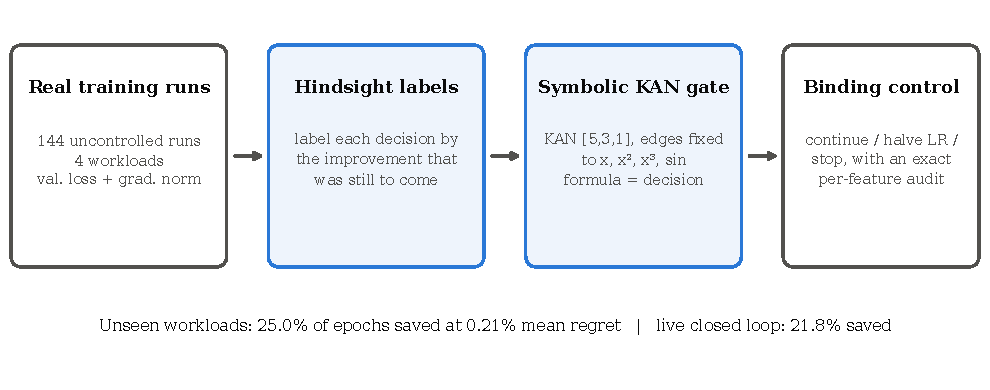
\includegraphics[width=\linewidth]{graphical_abstract.pdf}
\end{graphicalabstract}

\begin{keyword}
Kolmogorov--Arnold networks \sep early stopping \sep interpretable machine learning \sep learning-rate control \sep training orchestration \sep agentic systems
\end{keyword}


\end{frontmatter}

% ---------------------------------------------------------------- Specifications table
\section*{Specifications table}
\begin{center}
\small
\renewcommand{\arraystretch}{1.25}
\begin{tabularx}{\textwidth}{>{\bfseries}p{0.27\textwidth}X}
\toprule
Subject area & Computer Science \\
More specific subject area & Machine learning operations; interpretable control of neural network training (early stopping and learning-rate adjustment) \\
Name of your method & Hindsight-supervised symbolic KAN gate (HS-KAN gate) \\
Name and reference of original method & Kolmogorov--Arnold Networks: Z.~Liu, Y.~Wang, S.~Vaidya, F.~Ruehle, J.~Halverson, M.~Solja\v{c}i\'c, T.~Y.~Hou, M.~Tegmark, KAN: Kolmogorov--Arnold Networks, International Conference on Learning Representations (ICLR), 2025, arXiv:2404.19756. Early stopping: L.~Prechelt, Early stopping, but when?, in: Neural Networks: Tricks of the Trade, 2nd ed., Springer, 2012. \\
Resource availability & Source code, all recorded learning curves, trained gates, experiment outputs and the scripts that generate every table and figure: \url{https://github.com/avanishkasar/KAN-KubeAgent}. Software: Python 3.11, PyTorch, pykan 0.2.8, scikit-learn, SciPy, LangGraph. Data: Fashion-MNIST, MNIST and CIFAR-10 (public). Hardware: any computer; all results were produced on four CPU cores without a GPU. \\
\bottomrule
\end{tabularx}
\end{center}

% ---------------------------------------------------------------- Background
\section*{Background}
Training and fine-tuning jobs keep consuming compute long after they stop improving~\cite{schwartz2020greenai}. In practice they are supervised either by a person reading loss curves or by an automatic rule: patience on a validation signal~\cite{prechelt2012early}, the median stopping rule~\cite{golovin2017vizier}, or multi-fidelity schedulers such as successive halving, Hyperband~\cite{li2018hyperband}, ASHA~\cite{li2020asha} and BOHB~\cite{falkner2018bohb}, available in Optuna~\cite{akiba2019optuna}, Ray Tune~\cite{liaw2018tune} and the Kubernetes-native Katib~\cite{george2020katib}. Learning-curve extrapolation predicts a run's final performance from a partial curve with parametric ensembles~\cite{domhan2015extrapolation}, Bayesian neural networks~\cite{klein2017lcnet} or prior-data fitted networks~\cite{adriaensen2023lcpfn}. These methods save compute, but the reason a particular job was stopped is a rank, a quantile or a posterior rather than a statement an operator can check. Large language model (LLM) agents are now applied to the same task~\cite{zhang2023llmhpo,liu2024agenthpo,huang2024mlagentbench,chan2025mlebench}; they add natural-language rationales, but nothing guarantees that a rationale is what produced the action~\cite{yao2023react}.

For consequential automated decisions, models that are interpretable by construction are preferable to black boxes explained after the fact~\cite{rudin2019stop}. Kolmogorov--Arnold Networks (KANs)~\cite{liu2025kan} place learnable univariate functions on edges and can be converted into symbolic formulas~\cite{liu2024kan2}, which makes them a candidate for a controller whose decision rule can be read. Symbolic models have been used to explain hyperparameter optimisation after the fact~\cite{segel2023symbolic} and to distil learned optimisers~\cite{zheng2022symbolicl2o}, and KANs have produced interpretable reinforcement-learning policies~\cite{singh2025kanrl}. A controlled comparison finds that multilayer perceptrons generally match or exceed KANs except on symbolic-formula tasks~\cite{yu2024kanormlp}; we therefore claim no accuracy advantage for the KAN and compare it with linear, tree and MLP gates trained on identical labels. Placing a learned symbolic rule between an agent and the actions it may take also resembles shielding in safe reinforcement learning~\cite{alshiekh2018shielding}.

The method described here customises the original KAN method in two ways. First, it supplies a supervision signal for a control decision that has no ground truth at decision time: hindsight labels derived from completed runs (Step 3). Second, it turns the trained KAN into an executable closed-form decision rule and checks that the rule and the network agree (Step 4). It also adds a deployment guard against a failure mode we observed in closed-loop control (Step 5). The method was developed inside an agentic controller for Kubernetes training jobs, \texttt{KAN-KubeAgent}, but it does not depend on Kubernetes, on an LLM or on any particular training framework: it needs only per-epoch validation loss and gradient norm.

\paragraph{What was validated, and how}
We collected \nRuns{} complete, uncontrolled training runs (\nEpochsRecorded{} epochs) on four real workloads that differ in dataset, architecture and optimiser, and evaluated the gate against eleven alternatives with two protocols: cross-validation within each workload, grouped by seed, and leave-one-workload-out transfer, in which the gate controls a workload it has never seen. Uncertainty is reported with run-level bootstrap confidence intervals~\cite{efron1993bootstrap} and differences are tested with paired Wilcoxon signed-rank tests~\cite{wilcoxon1945} with Holm correction~\cite{holm1979}. We then let the gate control live training processes, including real learning-rate changes, on all four workloads. No synthetic or simulated data enters any result.

% ---------------------------------------------------------------- Method details
\section*{Method details}

\subsection*{Overview}
The method produces a \emph{gate}: a small function that reads five causal summary statistics of a running training job and returns a stop score $s\in[0,100]$. The score is mapped to one of three actions: continue ($s<40$), halve the learning rate ($40\le s<75$) or stop the job ($s\ge75$). The gate is a Kolmogorov--Arnold Network (KAN)~\cite{liu2025kan} whose edges are replaced, after training, by closed-form univariate functions, so the gate \emph{is} an algebraic expression that an operator can read, recompute and audit. It is trained by \emph{hindsight supervision}: every decision point of a completed training run is labelled with the improvement in validation loss that was actually still to come. Fig.~\ref{fig:overview} shows the five steps; each is specified below, followed by a step-by-step procedure and the exact commands that reproduce every number in this article.

\begin{figure}[t]
\centering
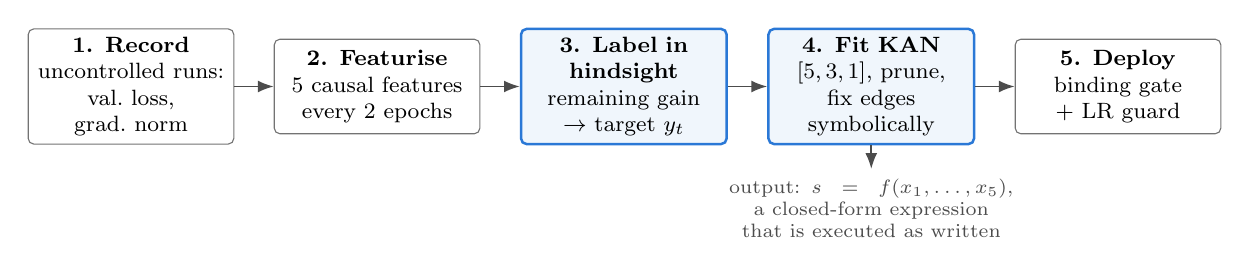
\begin{tikzpicture}[font=\footnotesize, node distance=4mm and 5mm,
  box/.style={draw=black!55, rounded corners=2pt, minimum height=12mm, text width=24mm, align=center, inner sep=3pt, fill=white},
  key/.style={box, draw=kblue, line width=0.9pt, fill=kblue!7},
  arr/.style={-{Latex[length=2mm]}, black!70, line width=0.6pt}]
\node[box] (s1) {\textbf{1. Record}\\uncontrolled runs:\\val.\ loss, grad.\ norm};
\node[box, right=of s1] (s2) {\textbf{2. Featurise}\\5 causal features\\every 2 epochs};
\node[key, right=of s2] (s3) {\textbf{3. Label in hindsight}\\remaining gain\\$\rightarrow$ target $y_t$};
\node[key, right=of s3] (s4) {\textbf{4. Fit KAN}\\$[5,3,1]$, prune,\\fix edges symbolically};
\node[box, right=of s4] (s5) {\textbf{5. Deploy}\\binding gate\\+ LR guard};
\draw[arr] (s1) -- (s2); \draw[arr] (s2) -- (s3); \draw[arr] (s3) -- (s4); \draw[arr] (s4) -- (s5);
\node[below=3mm of s4, text width=60mm, align=center, font=\scriptsize, text=black!70] (out) {output: $s=f(x_1,\dots,x_5)$, a closed-form expression\\that is executed as written};
\draw[arr, dashed] (s4) -- (out);
\end{tikzpicture}
\caption{The five steps of the method. Steps 3 and 4 (highlighted) are the customisation of the original KAN method; steps 1, 2 and 5 adapt standard early-stopping practice.}
\label{fig:overview}
\end{figure}

\subsection*{Step 1: record uncontrolled learning curves}
Train a set of runs of the target kind of job to their full epoch budget $T$ with no intervention, and record per epoch $t$ the validation loss $v_t$, the mean global $\ell_2$ gradient norm $g_t$ over the epoch's mini-batches, the validation accuracy and the wall-clock time. The validation loss must come from data the model never trains on. Vary the settings that change the shape of a curve (learning rate, batch size, random seed), because the gate learns from the variety of curve shapes, not from any single run. In this article $T=40$ and each workload contributes 36 runs (six learning rates $\times$ two batch sizes $\times$ three seeds; Table~\ref{tab:workloads}).

\subsection*{Step 2: compute five causal features}
At decision epoch $t$ the gate may use only $v_{1:t}$ and $g_{1:t}$. With a window of $w=5$ epochs, let $W_t=(v_{t-w+1},\dots,v_t)$ and $\Delta_i$ the successive differences inside $W_t$. The five features, each in $[0,1]$, are
\begin{align}
x_1 &= \operatorname{clip}\!\Big(1-10\,\frac{\max(v_{t-w+1}-v_t,\,0)}{|v_{t-w+1}|}\Big) && \text{plateau score}\label{eq:f1}\\
x_2 &= \operatorname{clip}\!\Big(\frac{\tfrac1w\sum_{s=t-w+1}^{t} g_s}{\max_{s\le t} g_s}\Big) && \text{gradient trend}\label{eq:f2}\\
x_3 &= \frac{\#\{i:\Delta_i\Delta_{i+1}<0\}}{w-2} && \text{oscillation (LR-decay benefit)}\label{eq:f3}\\
x_4 &= 1-t/T && \text{budget remaining}\label{eq:f4}\\
x_5 &= \operatorname{clip}\!\big((t-\arg\min_{s\le t} v_s)/30\big) && \text{epochs since improvement}\label{eq:f5}
\end{align}
where $\operatorname{clip}(\cdot)$ clips to $[0,1]$ and the window is truncated to the epochs available when $t<w$. Normalising the gradient norm by the run's own peak (Eq.~\ref{eq:f2}) makes $x_2$ scale-free across architectures, whose raw gradient norms differ by orders of magnitude. $x_3$ counts direction changes of the loss, a sign that a smaller learning rate may help. In the software the budget feature is named \texttt{gpu\_hours\_remaining\_vs\_budget}; in all experiments here it is the fraction of the epoch budget left, not a measured GPU-hour figure. Decisions are taken every two epochs from epoch 4, i.e.\ at $t\in\{4,6,\dots,38\}$, giving 18 decision points per run.

\subsection*{Step 3: label every decision point in hindsight}
Let $m_t=\min_{s\le t}v_s$ be the best validation loss seen by epoch $t$. Because the recorded run continued to $T$, the relative improvement that was still to come is known:
\begin{equation}
r_t=\frac{m_t-m_T}{m_t}\ \ge 0 .
\label{eq:gain}
\end{equation}
The training target for the decision point is
\begin{equation}
y_t=100\cdot\operatorname{clip}\!\big(1-r_t/\tau\big),
\label{eq:target}
\end{equation}
with tolerance $\tau=5\%$. A point with at least $\tau$ of improvement ahead receives $y_t=0$ (keep training); a point after which the run never improves again receives $y_t=100$ (stop now). With the decision bands above, a stop ($y_t\ge75$) means that less than $\tau/4=1.25\%$ relative improvement remained. The labels use the future only at training time; the features never do.

This step is the central customisation. The original agentic controller trained its gate to imitate a hand-written three-rule policy, which caps the gate at the quality of that rule, and re-labelled live runs with the gate's own past decisions, which is self-distillation and adds no information. Hindsight labels instead measure what each decision would actually have cost or saved.

\subsection*{Step 4: fit a KAN and fix its edges to symbolic functions}
The gate is a KAN of width $[5,3,1]$ with B-spline edges (grid size 5, order $k=3$), implemented with \texttt{pykan} 0.2.8. A KAN replaces each weight of a multilayer perceptron with a learnable univariate function on the edge and sums at the nodes~\cite{liu2025kan}, following the Kolmogorov--Arnold representation~\cite{kolmogorov1957}; its output here is
\begin{equation}
s(\mathbf{x})=\sum_{j=1}^{3}\phi^{(2)}_{j}\Big(\sum_{i=1}^{5}\phi^{(1)}_{j,i}(x_i)\Big).
\label{eq:kan}
\end{equation}
Fitting regresses $s$ on the targets $y_t$ with mean squared error, using Adam for 200 steps with an $\ell_1$ sparsity penalty $\lambda=0.01$ and entropy penalty 2.0, an 80/20 split of the training decision points for monitoring, pruning of inactive nodes and edges, and a 40-step refit of the pruned network. Then every remaining edge function is replaced by the best-fitting function from the library $\{x, x^2, x^3, \sin\}$ with fitted affine parameters (\texttt{auto\_symbolic}), and the expression is expanded with SymPy. After this step the network computes exactly the extracted expression: the formula shown to an operator is the decision function, not an approximation of it. We verify this on every gate by evaluating the network and the formula on the same inputs (\emph{faithfulness}, reported in Method validation).

The library is deliberately narrow. Exponentials, logarithms and nested compositions fit slightly better but produce expressions that are not readable at a glance, which defeats the purpose; the width $[5,3,1]$ is chosen for the same reason.

\subsection*{Step 5: deploy the gate as the binding decision layer}
In the released controller (\texttt{KAN-KubeAgent}) a LangGraph pipeline observes a running job, computes the features and lets a supervisor agent (a large language model when an API key is configured, otherwise a rule-based fallback) propose an action with a rationale. The proposal is advisory: the gate's band decision is what the executor carries out. \emph{Continue} is a no-op, \emph{adjust learning rate} halves the job's learning rate at the next epoch boundary, and \emph{early stop} terminates the job. Every decision is logged with the features, the score, the formula and an exact additive breakdown of the score into per-feature contributions.

A plateaued job keeps scoring in the adjust band, and an unguarded executor halves its learning rate at every decision point. We therefore add a \emph{learning-rate guard}: an adjustment is executed only if at least two decision points have passed since the previous one, and at most three times per job; a blocked adjustment is logged as deferred and the job continues unchanged. The effect of the guard is measured in closed-loop runs below.

\subsection*{Step-by-step procedure}
\begin{enumerate}
\item Install Python 3.10 or newer and the dependencies: \texttt{pip install -r training/requirements.txt -r kan\_gate/requirements.txt -r agents/requirements.txt -r dashboard/backend/requirements.txt}. A GPU is optional; every experiment here ran on four CPU cores.
\item Record curves for each workload (Step 1):\\ \texttt{python -m experiments.collect\_curves --workload fmnist\_cnn --epochs 40 --parallel 2}\\ and likewise for \texttt{mnist\_cnn}, \texttt{cifar10\_cnn} and \texttt{fmnist\_mlp\_sgd}. Each run is a subprocess of the same training script the live controller uses.
\item Evaluate (Steps 2 to 4 inside every fold): \texttt{python -m experiments.generalization} (both protocols, all baselines, sweeps, ablations) and \texttt{python -m experiments.benchmark} (the original single-workload benchmark).
\item Run closed-loop control: \texttt{python -m experiments.closed\_loop --workload <w> --gate lowo} for each workload, \texttt{--no-guard} for the unguarded executor.
\item Train the deployable gate on all recorded curves: \texttt{python -m kan\_gate.train --curves experiments/data/curves*.jsonl}. The learned formula is printed and the checkpoint saved.
\item Start the controller and dashboard with \texttt{./start.sh} (Linux, macOS) or \texttt{.\textbackslash start.ps1} (Windows) and open \url{http://localhost:8000}.
\item Regenerate the tables, numbers and figures of this article: \texttt{python -m experiments.paper\_methodsx}.
\end{enumerate}
To apply the method to a new kind of job, repeat steps 2 to 5 with curves of that job; to use it without retraining, use a gate trained on other workloads, which is what the leave-one-workload-out protocol below evaluates.

% Method validation
% ---------------------------------------------------------------- Method validation: setup
\section*{Method validation}

\subsection*{Workloads and recorded runs}
We recorded \nRuns{} complete training runs on four workloads (Table~\ref{tab:workloads}). Each workload is a grid of six learning rates, two batch sizes (64, 256) and three seeds (0, 1, 2), trained for $T=\X{budget}$ epochs on a fixed 4{,}000-image subset of the official training split, with validation loss and accuracy measured after every epoch on 2{,}000 images of the official test split. The CNN workloads use Adam~\cite{kingma2015adam}; the MLP workload uses SGD with momentum 0.9~\cite{sutskever2013momentum}, so that the gate also meets an optimiser whose curves look different. The learning-rate grids span stable, fast and unstable training: some runs are still improving at epoch 40, others overfit within a few epochs, and some diverge or stall (Fig.~\ref{fig:curves}). All runs use the same PyTorch~\cite{paszke2019pytorch} training script that the controller launches in deployment, with in-process data loading and two CPU threads per run. Re-running a configuration with the same seed reproduces its recorded curve exactly; we checked this for the first two epochs of the first Fashion-MNIST run, whose losses matched the stored values bit for bit.

\begin{table}[t]
\centering
\caption{The four workloads. Each has 36 uncontrolled runs (6 learning rates $\times$ 2 batch sizes $\times$ 3 seeds, 40 epochs). Accuracy is the median over runs of the best validation accuracy; ``best epoch'' is the median epoch of minimum validation loss; ``late'' is the share of runs whose minimum falls in the last five epochs; time is the mean wall-clock time per epoch on two CPU threads.}
\label{tab:workloads}
\footnotesize
\setlength{\tabcolsep}{4pt}
\begin{tabular}{llllrrrr}
\toprule
Dataset & Model & Optimiser & Learning rates & Acc.\ (\%) & Best ep. & Late (\%) & s/ep. \\
\midrule
\tabinput{generated/table_workloads.tex}
\bottomrule
\end{tabular}
\end{table}

\begin{figure}[t]
\centering
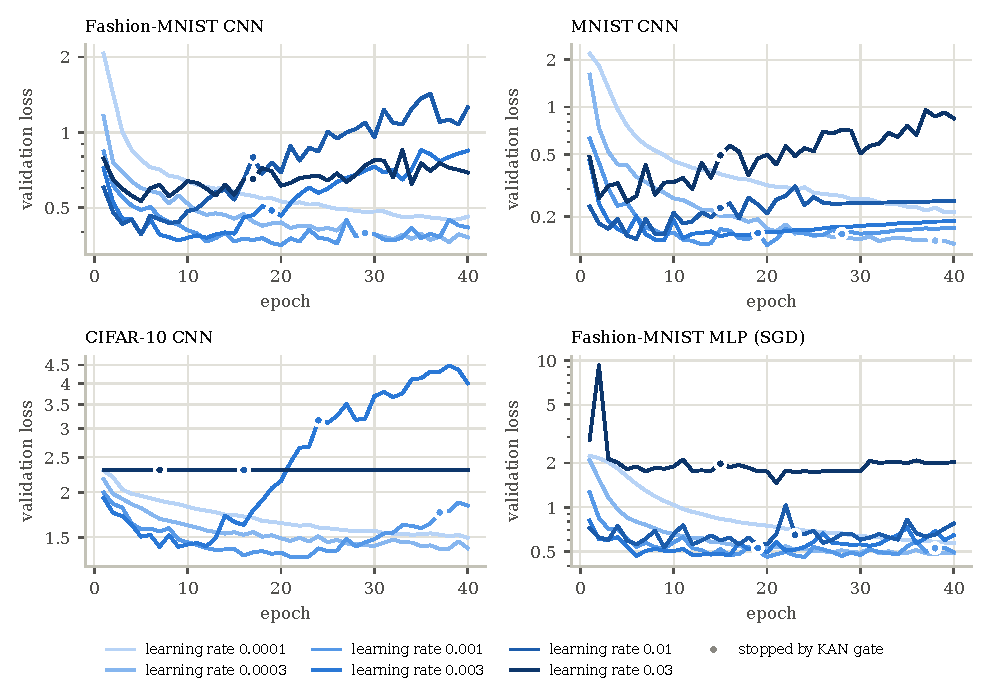
\includegraphics[width=\textwidth]{figures/curves.pdf}
\caption{Validation loss of the six learning rates (batch size 64, seed 2) on each workload, log scale. Dots mark where the KAN gate trained on the \emph{other three} workloads stops each run (leave-one-workload-out, mean over three gate seeds); runs without a dot were trained to the full budget.}
\label{fig:curves}
\end{figure}

\subsection*{Evaluation protocol}
\paragraph{Counterfactual replay} Every stopping policy is replayed on the recorded curves: at each decision epoch $t\in\{4,6,\dots,38\}$ the policy sees the run's history up to $t$ and either continues or stops. A policy that stops at epoch $t$ is credited with the best validation loss observed up to $t$, which is what a practitioner who checkpoints the best model obtains. Because a learning-rate change alters the future of a run, \emph{adjust} decisions are treated as \emph{continue} in replay and evaluated in the closed-loop experiments instead.

\paragraph{Metrics} For each run, \emph{compute saved} is $1-t_{\text{stop}}/T$, averaged over runs. \emph{Regret} is the relative excess of the best validation loss obtained over the best validation loss of the full run, $(m_{t_{\text{stop}}}-m_T)/m_T$; we report its mean, its 90th percentile and its maximum. A stop with regret above 2\% is counted as \emph{premature}. We also report the drop in validation accuracy (percentage points) at the best checkpoint.

\paragraph{Policies} The gate (KAN, hindsight labels) is compared with: (i) the same hindsight labels fitted by ridge regression (\emph{linear}), a depth-3 regression tree and a two-layer MLP (32--32) from scikit-learn~\cite{pedregosa2011sklearn}, all using the same features and the same decision bands; (ii) the same KAN trained on the same decision points but labelled by the hand-written three-rule policy of the original controller instead of in hindsight (\emph{rule labels}), which isolates the effect of the label source, and that rule itself; (iii) patience rules with patience 3, 5 and 8 epochs~\cite{prechelt2012early}; (iv) the median stopping rule~\cite{golovin2017vizier}, which stops a run whose best loss is worse than the median of the running-average losses of completed runs of the same workload with other seeds at the same epoch; (v) no early stopping; and (vi) a hindsight oracle that stops at the first decision epoch at which less than 1.25\% relative improvement remains, an upper reference that no causal policy can reach.

\paragraph{Protocols} \emph{Within-workload}: three-fold cross-validation inside each workload with folds grouped by seed, so that no test run, and no run sharing a test run's initialisation, is seen in training. \emph{Leave-one-workload-out (LOWO)}: learned gates are trained on all runs of three workloads and tested on every run of the fourth, the situation of a practitioner who deploys a gate on a new kind of job without collecting curves first. Every learned gate is fitted with three seeds (0, 1, 2) and the per-run outcome is averaged over seeds. A learned gate is trained on 432 decision points (24 runs) per fold within a workload and on 1{,}944 decision points (108 runs) in LOWO.

\paragraph{Statistics} Confidence intervals are 95\% percentile intervals from \X{nBoot} bootstrap resamples of runs~\cite{efron1993bootstrap}. Differences between the KAN gate and each alternative are tested per run (\nRuns{} pairs) with the two-sided Wilcoxon signed-rank test~\cite{wilcoxon1945}, zero differences split between ranks, and $p$-values are Holm-corrected~\cite{holm1979} across the nine comparisons of each metric and protocol.

% ---------------------------------------------------------------- Method validation: offline results
\subsection*{Offline results}
Table~\ref{tab:main} lists every policy under both protocols, and Fig.~\ref{fig:frontier} places the learned gates and the patience rule on the trade-off between compute saved and regret. Four observations follow.

\paragraph{The gate transfers to unseen workloads} Trained on three workloads and applied to the fourth, the KAN gate saved \R{lowo}{kan}{saved}\% of all epochs (95\% CI \R{lowo}{kan}{savedlo} to \R{lowo}{kan}{savedhi}) at a mean regret of \R{lowo}{kan}{regret}\% (CI \R{lowo}{kan}{regretlo} to \R{lowo}{kan}{regrethi}), with \R{lowo}{kan}{prem}\% of runs stopped prematurely and a mean accuracy loss of \R{lowo}{kan}{acc} percentage points. Within a workload it saved \R{within}{kan}{saved}\% at \R{within}{kan}{regret}\% regret with \R{within}{kan}{prem}\% premature stops, so moving to an unseen workload cost no quality and about two percentage points of savings. Transfer works because every feature is normalised per run: a gate learns what a plateau looks like, not the loss level of a particular dataset. Of all learned gates, the KAN had the lowest mean regret and premature-stop rate under transfer (Table~\ref{tab:main}); the MLP and the depth-3 tree saved more compute but stopped \R{lowo}{mlp}{prem}\% and \R{lowo}{tree}{prem}\% of runs prematurely, and their regret was significantly higher ($p\T{lowo}{mlp}{regret}{p}$ and $p\T{lowo}{tree}{regret}{p}$, Table~\ref{tab:tests}).

\paragraph{Hindsight labels are what make the gate useful} The same KAN, trained on the same real decision points but with the labels of the hand-written rule, saved only \R{lowo}{kanrule}{saved}\% under transfer (\R{within}{kanrule}{saved}\% within workloads) and stopped runs significantly later ($p\T{lowo}{kanrule}{stop}{p}$), with no significant difference in regret ($p\T{lowo}{kanrule}{regret}{p}$). The rule itself, applied directly, stopped \R{lowo}{rule}{prem}\% of runs prematurely. Imitating a rule therefore produces a cautious copy of the rule's thresholds, while hindsight labels produce a gate that stops when the remaining improvement is actually small.

\paragraph{A well-chosen patience rule is as good on the stopping axis} Patience 8 saved \R{lowo}{pateight}{saved}\% at \R{lowo}{pateight}{regret}\% regret, and the regret of the KAN gate is not significantly different from it ($p\T{lowo}{pateight}{regret}{p}$); patience stopped slightly earlier ($p\T{lowo}{pateight}{stop}{p}$). On the frontier of Fig.~\ref{fig:frontier} the patience family and the linear gate lie at or slightly above the KAN gate's curve, i.e.\ for the stop decision alone they reach the same regret with a few percentage points more compute saved. Shorter patience is clearly worse: patience 3 stopped \R{lowo}{patthree}{prem}\% of runs prematurely. The median stopping rule had a mean regret of \R{lowo}{median}{regret}\%, because in a grid of learning rates it stops slow-starting configurations that later become the best; it is designed for comparing trials, not for deciding when a single job has finished. The value of the KAN gate is therefore not a better stopping trade-off than a tuned patience rule. It is that a single learned rule, with no per-workload tuning, makes calibrated stop decisions on unseen workloads, also decides when to adjust the learning rate, and is an explicit formula whose every decision can be recomputed and attributed.

\paragraph{Every workload behaves consistently} Table~\ref{tab:perworkload} breaks the transfer result down by held-out workload. The KAN gate kept mean regret at or below 0.6\% on every held-out workload, including CIFAR-10, the only colour-image workload, and the SGD-trained MLP, the only workload with a different optimiser. Its largest single-run regret, \R{lowo}{kan}{max}\%, occurs on one unstable SGD run (learning rate 0.3) whose validation loss hovers without progress for about 15 epochs and then reaches its best value in a single isolated dip at epoch 21; every hindsight-trained gate and both patience 5 and patience 8 stop that run before the dip, and only the oracle does not.

\begin{table}[p]
\centering
\caption{Offline replay on \nRuns{} real runs. Compute saved and mean regret with 95\% bootstrap confidence intervals; ``prem.'' is the share of runs stopped with more than 2\% regret. Within: seed-grouped 3-fold cross-validation inside each workload. LOWO: trained on three workloads, tested on the fourth. Policies without training (patience, median rule, rule, oracle, no stopping) are identical under both protocols.}
\label{tab:main}
\footnotesize
\setlength{\tabcolsep}{3.5pt}
\resizebox{\textwidth}{!}{%
\begin{tabular}{lrrrrrr}
\toprule
& \multicolumn{3}{c}{Within-workload} & \multicolumn{3}{c}{Leave-one-workload-out} \\
\cmidrule(lr){2-4}\cmidrule(lr){5-7}
Policy & Saved (\%) & Regret (\%) & Prem.\ (\%) & Saved (\%) & Regret (\%) & Prem.\ (\%) \\
\midrule
\tabinput{generated/table_main.tex}
\bottomrule
\end{tabular}}
\end{table}

\begin{figure}[p]
\centering
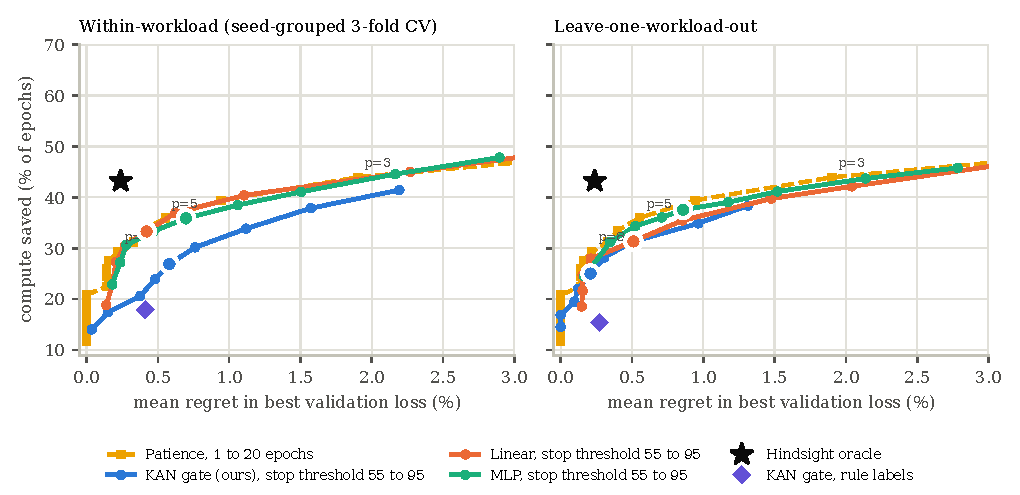
\includegraphics[width=\textwidth]{figures/frontier.pdf}
\caption{Trade-off between compute saved and mean regret. Learned gates are traced by sweeping the stop threshold from 55 to 95 (large dot: the deployed threshold 75); the dashed line is the patience rule for patience 1 to 20 epochs. Points further up and to the left are better. The median stopping rule (mean regret \R{lowo}{median}{regret}\%) lies outside the plotted range.}
\label{fig:frontier}
\end{figure}

\begin{table}[t]
\centering
\caption{Leave-one-workload-out results per held-out workload: compute saved (\%) / mean regret (\%).}
\label{tab:perworkload}
\footnotesize
\resizebox{\textwidth}{!}{%
\begin{tabular}{lcccc}
\toprule
Policy & Fashion-MNIST CNN & MNIST CNN & CIFAR-10 CNN & F-MNIST MLP (SGD) \\
\midrule
\tabinput{generated/table_per_workload.tex}
\bottomrule
\end{tabular}}
\end{table}

\begin{table}[t]
\centering
\caption{Paired comparison of the KAN gate with each alternative over \nRuns{} runs: median difference (KAN minus alternative) in stop epoch and in regret (percentage points), with Holm-corrected Wilcoxon signed-rank $p$-values. A negative stop difference means the KAN gate stops earlier.}
\label{tab:tests}
\footnotesize
\setlength{\tabcolsep}{4pt}
\resizebox{\textwidth}{!}{%
\begin{tabular}{lrrrrrrrr}
\toprule
& \multicolumn{4}{c}{Within-workload} & \multicolumn{4}{c}{Leave-one-workload-out} \\
\cmidrule(lr){2-5}\cmidrule(lr){6-9}
Alternative & $\Delta$stop & $p$ & $\Delta$regret & $p$ & $\Delta$stop & $p$ & $\Delta$regret & $p$ \\
\midrule
\tabinput{generated/table_tests.tex}
\bottomrule
\end{tabular}}
\end{table}

\subsection*{Ablations}
Table~\ref{tab:ablation} repeats the leave-one-workload-out evaluation with one feature at a time replaced by its training mean, and with three hindsight tolerances. Epochs since improvement ($x_5$) carries most of the decision: without it the gate stops much earlier and regret rises from \A{none}{regret}\% to \A{x5}{regret}\%. The plateau score ($x_1$) and the oscillation feature ($x_3$) each add a few percentage points of compute saved at unchanged regret; gradient trend ($x_2$) and budget remaining ($x_4$) change little on these workloads. The tolerance $\tau$ is a direct and predictable control of the trade-off: $\tau=2\%$ gives \Sw{2}{saved}\% saved at \Sw{2}{regret}\% regret and $\tau=10\%$ gives \Sw{10}{saved}\% at \Sw{10}{regret}\%, so an operator sets the acceptable loss of quality in the units in which it is measured.

\begin{table}[t]
\centering
\caption{Feature ablation and tolerance sweep, leave-one-workload-out, KAN gate (three gate seeds). Top: one feature replaced by its training-set mean in training and test. Bottom: hindsight tolerance $\tau$ (default 5\%).}
\label{tab:ablation}
\small
\begin{tabular}{lrrr}
\toprule
Feature removed / setting & Saved (\%) & Regret (\%) & Premature (\%) \\
\midrule
\tabinput{generated/table_ablation.tex}
\bottomrule
\end{tabular}
\end{table}

% ---------------------------------------------------------------- Method validation: interpretability
\subsection*{The gate is an exact, readable formula}
\paragraph{Faithfulness} For each of the \X{nGates} KAN gates fitted in the two protocols we evaluated the network and its extracted formula on the same test decision points. The largest absolute difference over all gates and points was $\X{faithMax}$ score points on the 0 to 100 scale (median over gates $\X{faithMed}$), i.e.\ floating-point agreement: the formula is the decision function. The median gate kept \X{edgesMed} active edges after pruning and its expanded formula has \X{termsMed} additive terms (largest \X{termsMax}).

\paragraph{The price of readability} Fixing the spline edges to symbolic functions is not free. On the held-out 20\% of each gate's training decision points, the mean absolute error of the stop score against the hindsight target rose from \X{maeSpline} points for the spline network to \X{maeSymbolic} points for the symbolic gate. Because the gate is used only through three wide decision bands, this loss of fit costs little in decisions (Table~\ref{tab:main}), but users who need a more precise score should keep the spline network and report its symbolic approximation instead, at the cost of exactness.

\paragraph{The deployed gate} Trained on all \nRuns{} runs (\X{depRows} decision points), the gate shipped with the controller is
\begin{equation}
s = 21.86 x_1 - 19.3 x_2 + 20.33 x_3 - 14.61 x_4 + 72.24 x_5 - 3.77 \sin{(1.49 x_3 + 6.51 )} + 34.99

\label{eq:deployed}
\end{equation}
with $x_1,\dots,x_5$ as in Eqs.~(\ref{eq:f1})--(\ref{eq:f5}), coefficients rounded to two decimals for display (the controller evaluates the unrounded expression; network and formula agree to $\X{depFaith}$ points on all recorded decision points). Fig.~\ref{fig:edges} shows each of its \X{depActiveEdges} active edge functions. An operator can read the gate's behaviour directly from Eq.~(\ref{eq:deployed}): which features push towards stopping, which towards continuing, and by how much; and for any logged decision the controller reports the score's per-feature contributions, computed from the gate itself.

\begin{figure}[t]
\centering
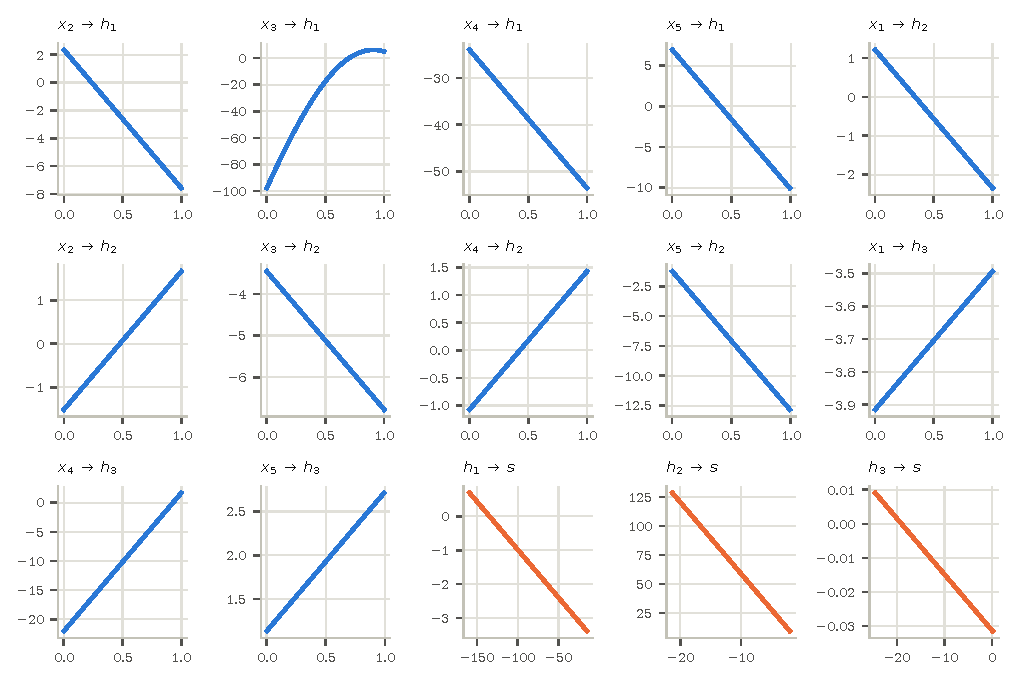
\includegraphics[width=\textwidth]{figures/edges.pdf}
\caption{Active edge functions of the deployed gate after symbolic fixing, each drawn over the range of inputs it receives on the recorded decision points. Blue: first layer (feature $x_i$ to hidden node $h_j$); orange: second layer (hidden node to stop score $s$).}
\label{fig:edges}
\end{figure}

\paragraph{Cost} Fitting a gate, including pruning and symbolic extraction, took \X{fitSeconds} s on average on a CPU, and one decision takes about \X{latKan} ms in pykan, negligible against a training epoch. Evaluating the extracted expression directly, as the static web preview of the controller does in the browser, is cheaper still.

% ---------------------------------------------------------------- Method validation: closed loop
\subsection*{Closed-loop control of live training}
Offline replay cannot show what a learning-rate change does. We therefore let the complete controller (feature extraction, supervisor, gate, executor) control live training processes. For each workload we re-ran the 12 configurations of seed 2 under control, with the gate trained on the \emph{other three} workloads, and compared each controlled run with its uncontrolled recording, which has the same seed and settings. Control is asynchronous, as in deployment: the process keeps training while the controller decides, and a learning-rate change takes effect at the next epoch boundary. Until the first intervention, every controlled run reproduced its uncontrolled curve, which confirms that the comparison is paired.

\begin{table}[t]
\centering
\caption{Closed-loop control of live training (12 configurations of seed 2 per row). Top: gates trained on the other three workloads, with the learning-rate guard. Bottom: effect of the guard. ``Change'' is the relative change in best validation loss against the same run uncontrolled (negative is better); ``worse'' counts runs more than 2\% worse; $p$ is the Wilcoxon signed-rank test of controlled against uncontrolled best validation loss; the last column gives learning-rate halvings in total and (in brackets) the most in one run.}
\label{tab:closed}
\footnotesize
\setlength{\tabcolsep}{3.5pt}
\resizebox{\textwidth}{!}{%
\begin{tabular}{lrrrrrrrr}
\toprule
Workload / condition & Runs & Epochs used & Saved (\%) & Median change (\%) & Min / max (\%) & Worse & $p$ & LR halvings \\
\midrule
\multicolumn{9}{l}{\emph{Unseen-workload gate, guard on}}\\
\tabinput{generated/table_closed_lowo.tex}
\midrule
\multicolumn{9}{l}{\emph{Learning-rate guard off versus on}}\\
\tabinput{generated/table_closed_guard.tex}
\bottomrule
\end{tabular}}
\end{table}

\begin{figure}[t]
\centering
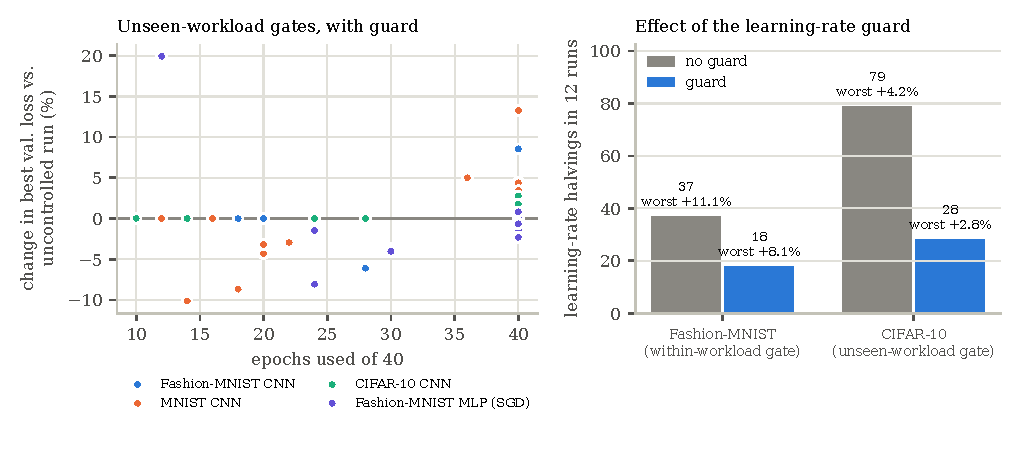
\includegraphics[width=\textwidth]{figures/closed_loop.pdf}
\caption{Closed-loop control. Left: for each of the 48 live runs controlled by a gate that had never seen its workload, epochs used and the change in best validation loss against the same run uncontrolled. Right: learning-rate halvings over 12 runs without and with the guard, and the worst single-run change in best validation loss.}
\label{fig:closed}
\end{figure}

\paragraph{Unseen workloads} Over all 48 runs the controller used \C{lowoall}{used} of \C{lowoall}{budget} epochs (\C{lowoall}{saved}\% saved) and stopped \C{lowoall}{stopped} runs early (Table~\ref{tab:closed}, Fig.~\ref{fig:closed}). The best validation loss was unchanged in the median (\C{lowoall}{relmed}\%) and not significantly different from uncontrolled training ($p\C{lowoall}{p}$); \C{lowoall}{better} runs ended more than 2\% better and \C{lowoall}{worse} more than 2\% worse, and the mean change in validation accuracy at the best checkpoint was $\C{lowoall}{acc}$ percentage points. Savings were lower than in offline replay of the same 48 configurations (\X{offlineSeedTwoSaved}\%) because a run's curve changes after a learning-rate halving, so the controlled runs are no longer the recorded ones, and because a stop decided asynchronously takes effect only at the process's next epoch boundary. The largest loss, \C{lowomlpsgd}{relmax}\%, is the unstable SGD run discussed above, which the gate stopped before its isolated late minimum.

\paragraph{The learning-rate guard} Without the guard the executor halved the learning rate up to \C{fmnistnoguard}{adjmax} times in one Fashion-MNIST run and up to \C{cifarnoguard}{adjmax} times in one CIFAR-10 run, leaving those runs at a small fraction of their initial learning rate. With the guard, at most \C{fmnistguard}{adjmax} halvings per run were executed (\C{fmnistguard}{deferred} further requests were deferred on Fashion-MNIST), and the worst single-run change in best validation loss fell from $+\C{fmnistnoguard}{relmax}\%$ to $+\C{fmnistguard}{relmax}\%$ on Fashion-MNIST and from $+\C{cifarnoguard}{relmax}\%$ to $+\C{lowocifar}{relmax}\%$ on CIFAR-10, at the cost of fewer epochs saved on Fashion-MNIST (\C{fmnistguard}{saved}\% against \C{fmnistnoguard}{saved}\%). Neither condition changed best validation loss significantly. The guard is a deployment safeguard rather than a learned component, and its two parameters (spacing and maximum count) should be revisited for jobs with very different schedules.


% ---------------------------------------------------------------- Limitations
\section*{Limitations}
\begin{itemize}
\item \textbf{Scale of the workloads.} All runs are small image classifiers trained on 4{,}000-image subsets for 40 epochs on a CPU. Large models, long schedules with warm-up and decay, and fine-tuning of pretrained networks produce curve shapes that are not represented here; a gate for such jobs should be retrained on their curves (Steps 1 to 4), and its transfer should be checked with the leave-one-workload-out protocol before it is trusted.
\item \textbf{No accuracy advantage over simpler gates.} On the same hindsight labels a linear gate reaches a similar trade-off and patience rules with a well-chosen patience are competitive (Method validation). The contribution of the KAN is an exact, readable and non-linear decision rule, together with the training signal that makes such a rule useful; it is not higher accuracy. Where a linear rule is sufficient for a workload, it is also acceptable and even simpler to audit.
\item \textbf{Offline replay covers stopping only.} A recorded curve cannot show what a learning-rate change would have done, so the offline benchmark scores the stop decision and treats \emph{adjust} as \emph{continue}. Learning-rate adjustment is evaluated only in the closed-loop experiments, on 12 runs per condition.
\item \textbf{Hindsight labels need complete runs.} Runs that a gate itself stopped have no observed future and cannot be labelled; harvesting labels from a deployed gate is therefore right-censored. Collecting a share of uncontrolled runs, or runs continued past the gate's stop for a few epochs, avoids this bias.
\item \textbf{Budget feature.} The budget feature is the fraction of the epoch budget remaining, not measured accelerator time. Deployments with heterogeneous hardware should replace it with a measured quantity and retrain.
\item \textbf{Supervisor agent not evaluated.} All experiments ran with the rule-based fallback supervisor (no LLM). Because the gate is binding, the supervisor's proposal does not change any action; its rationales were not evaluated.
\item \textbf{Cluster deployment.} The released controller includes a Kubeflow Trainer client, but all reported runs used the local process client. Behaviour on a live Kubernetes cluster, such as scheduling delays between a decision and its effect, was not measured.
\end{itemize}

% ---------------------------------------------------------------- Statements
\section*{Ethics statements}
This work involved no human participants, no animal experiments and no data collected from social media platforms. All datasets used (Fashion-MNIST, MNIST, CIFAR-10) are public benchmark image collections, used under their published terms.

\section*{CRediT author statement}
\textbf{Avanish Kasar:} Conceptualization, Methodology, Software, Investigation, Formal analysis, Data curation, Visualization, Writing -- original draft.
\textbf{Rupali Biradar:} Validation, Writing -- review \& editing.
\textbf{Viverun:} Investigation, Validation, Writing -- review \& editing.

\section*{Data availability}
All data and code are openly available at \url{https://github.com/avanishkasar/KAN-KubeAgent}: the \nRuns{} recorded learning curves (\texttt{experiments/data/}), all experiment outputs (\texttt{experiments/results/}), the trained gates, and the script \texttt{experiments/paper\_methodsx.py} that regenerates every number, table and figure in this article.

\section*{Acknowledgements}
This research did not receive any specific grant from funding agencies in the public, commercial, or not-for-profit sectors.

\section*{Declaration of competing interests}
The authors declare that they have no known competing financial interests or personal relationships that could have appeared to influence the work reported in this paper.

\section*{Declaration of generative AI and AI-assisted technologies in the writing process}
During the preparation of this work the authors used AI-assisted tools to help draft text and software. After using these tools, the authors reviewed and edited the content as needed and take full responsibility for the content of the publication.


\bibliographystyle{elsarticle-num}
\bibliography{refs}

\end{document}
